\pagebreak
\section*{Appendix}

This appendix is formatted as follows.
\begin{enumerate}
    \item We discuss the \textit{Datasets and models} used in our work in Appendix~\ref{app:datasets}.
    \item We discuss \textit{Weight perturbation} and display full results from ablations in Appendix~\ref{app:weights}.
    \item We detail our \textit{Mode connectivity} implementation in Appendix~\ref{app:mode}.
    \item We display full \textit{Comparison of ensemble techniques} in Appendix~\ref{app:experiments}.
    \item We discuss \textit{Limitations and future work} in Appendix~\ref{app:limitations}.
\end{enumerate}
Where necessary, we discuss potential
limitations of our work and future avenues for exploration.

\section{Datasets and models}
\label{app:datasets}

Five benchmark datasets are employed in our experiments, all of which describe binary classification and are publicly available. Details are provided in Appendix~\ref{subapp:datasets} and in Table~\ref{tab:appdatasets}. Our experiments are also conducted for a fixed architecture, trained with hyperparameters determined through model selection sweeps. Details are provided in Appendix~\ref{subapp:models} and Table~\ref{tab:appmodels}.

\subsection{Datasets}
\label{subapp:datasets}

\begin{table*}[b]
\caption{\small Summary of the datasets used in our experiments. Although German Credit includes continuous features, we find that they have limited effect on the model both during training and in the resulting explanations.}
\label{tab:appdatasets}
\centering
\begin{tabular}{ccccccc}
\toprule
Name & No. Inputs & Input Dim. & Categorical & Continuous & No. Train & No. Test\\
\toprule
\midrule
HELOC & 9871 & 23 & 0 & 23 & 7896* & 1975*\\
\midrule
German Credit & 999 & 70* & 17 & 3 & 799 & 200\\
\midrule
Adult Income & 32561 & 6 & 0 & 6 & 26048 & 6513\\
\midrule
Default Credit & 30000 & 90* & 9 & 14 & 24000 & 6000\\
\midrule
GMSC & 11426 & 10 & 0 & 10 & 9140 & 2286\\
\toprule
\end{tabular}
\small *Denotes values post-processing (one-hot encoding inputs, dropping inputs).
\end{table*}

The \textbf{HELOC} (Home Equity Line of Credit) dataset \citep{heloc} classifies \textbf{credit risk} and can be obtained from (upon request) and is described in detail at: {\footnotesize\url{https://community.fico.com/s/explainable-machine-learning-challenge}}. We drop duplicate inputs, and inputs where all feature values are missing (negative), and replace remaining missing values in the dataset with median values.

The \textbf{German Credit} dataset \citep{uci2017} classifies \textbf{credit risk} and can be obtained from and is described at: {\footnotesize\url{https://archive.ics.uci.edu/ml/datasets/statlog+(german+credit+data)}}. The documentation for this dataset also details a cost matrix, where false positive predictions induce a higher cost than false negative predictions, but we ignore this in model training. Note that this dataset includes mostly categorical features, and is distinct from the common Default Credit dataset, described below.

The \textbf{Adult Income} dataset \citep{uci2017} classifies whether an individual's \textbf{salary} exceeds \$50,000, and is obtained from and described at: {\footnotesize\url{https://archive.ics.uci.edu/ml/datasets/adult}}. We drop categorical features for this dataset, resulting in a total of 6 features, to include an assessment of a case where \textit{top-5} would encompass most features (n.b., we still see significant disagreement in this case- either the signs of the 5 features disagreed, or the least important 6$^\text{th}$ feature was disagreed on).

The \textbf{Default Credit} dataset \citep{yeh2009} classifies \textbf{default risk} on customer payments and is obtained from and described at: {\footnotesize\url{https://archive.ics.uci.edu/ml/datasets/default+of+credit+card+clients}}. This dataset, and German Credit, stress-test increased dimensions (number of features). 

The \textbf{GMSC} (Give Me Some Credit) dataset \citep{gmsc} classifies the \textbf{probability of default} within the next two years, and is obtained from and described at: {\footnotesize\url{https://www.kaggle.com/datasets/brycecf/give-me-some-credit-dataset}}. We pre-process a large random sample of this dataset, ensuring a 50-50 split between class 0 (no default) and class 1 (default). Summary of these datasets is in Table~\ref{tab:appdatasets}.

\subsection{Models}
\label{subapp:models}

We use \verb+PyTorch+~\citep{paszke2019} to implement feedforward neural networks with fixed architectures: hidden layers of size 128, 64, and 16. We use ReLU activations for the intermediate layers and Softmax for the output. Model selection sweeps are performed with \verb+RayTune+ \citep{liaw2018}, to identify the best performing model hyperparameters for a given dataset (shown in Table~\ref{tab:appmodels}). We performed iterative searches across learning rates from $10^{-6}$ to $10^{-1}$, batch sizes 16 to 128, and epochs typically between 5 and 100 (though only larger values where necessary). Notably, there were a wide range of hyperparameters that yielded near equivalent \textit{test accuracy}. The investigation of ensembling techniques should be extended to the Rashomon set for a given architecture and, further, across various model sizes. Our research focused on the natural starting point of analyzing a given underspecification set, where the ML pipeline is optimized up until the choice of the random seed used in training. We employ a filtering process to discard models that perform more than 1\% below the mean accuracy, though also recognize the importance of seed-induced variability in the context of automated systems. If the focus is on investigating the effects of random seeds, it could be argued that all models should be included. We initially tested both approaches, and found the overall trends in the results to be largely similar.

\begin{table*}[t]
\caption{\small Hyperparameters used to train our models, and model performance.}
\label{tab:appmodels}
\centering
\begin{tabular}{cccccc}
\toprule
Name & Epochs & Learning Rate & Batch Size & Train Acc. (\%) & Test Acc. (\%)\\
\toprule
\midrule
HELOC & 20 & 0.0004 & 32 & 77.97 $\pm$ 0.31 & 72.90 $\pm$ 0.45\\
\midrule
German Credit & 100 & 0.004 & 32 & 92.81 $\pm$ 1.98 & 73.47 $\pm$ 1.47\\
\midrule
Adult Income & 40 & 0.004 & 128 & 83.50 $\pm$ 0.15 & 82.12 $\pm$ 0.16\\
\midrule
Default Credit & 10 & 0.0001 & 128 & 82.32 $\pm$ 0.05 & 82.67 $\pm$ 0.09\\
\midrule
GMSC & 20 & 0.0004 & 32 & 75.17 $\pm$ 0.34 & 73.96 $\pm$ 0.34\\
\bottomrule
\end{tabular}
\end{table*}


\section{Weight perturbation}
\label{app:weights}

\begin{figure}[b]
    \centering
    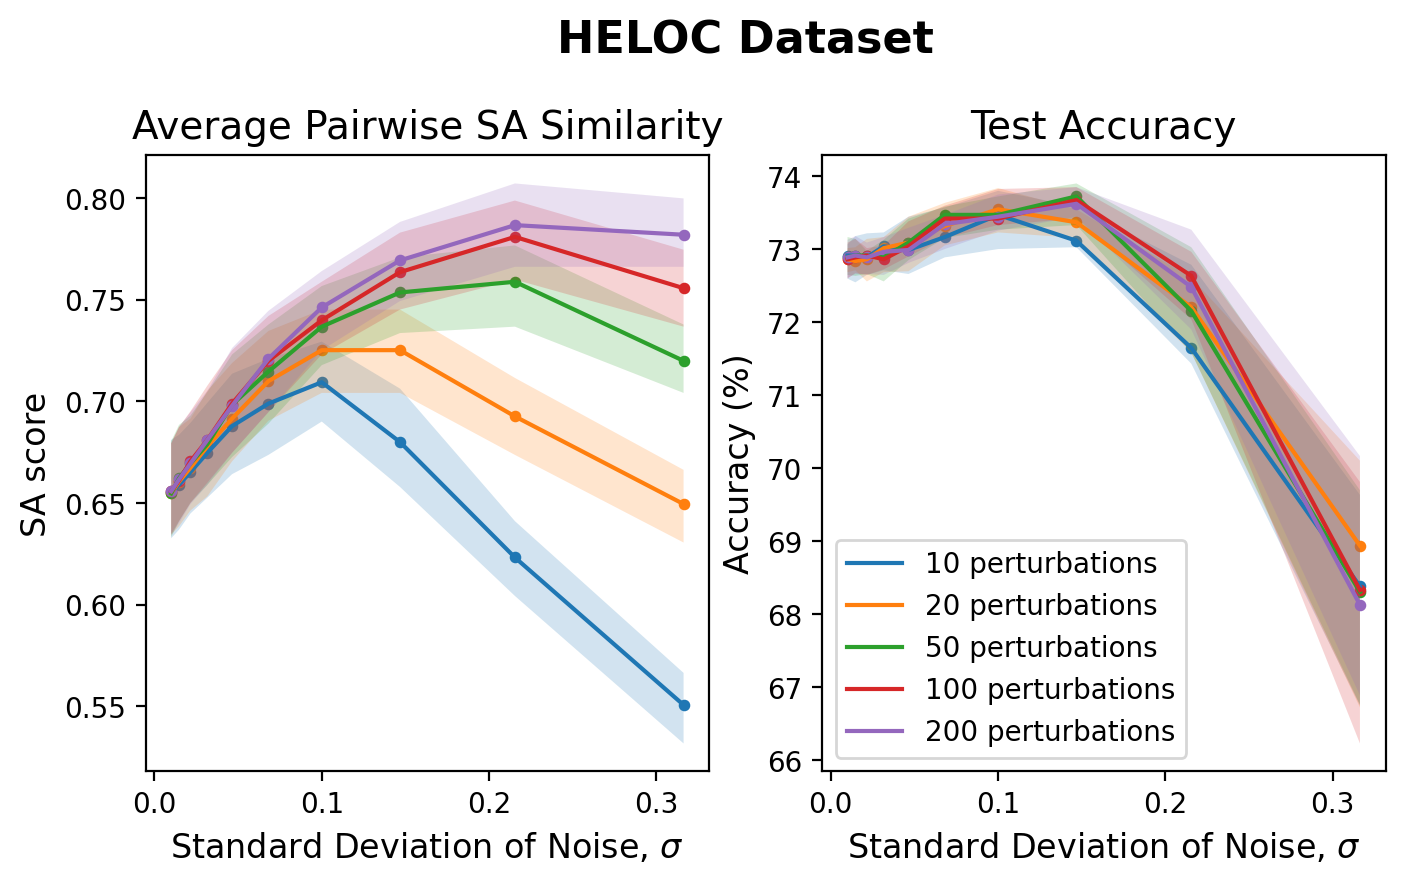
\includegraphics[width=0.325\textwidth]{figures/perturb_heloc_samples.png}
    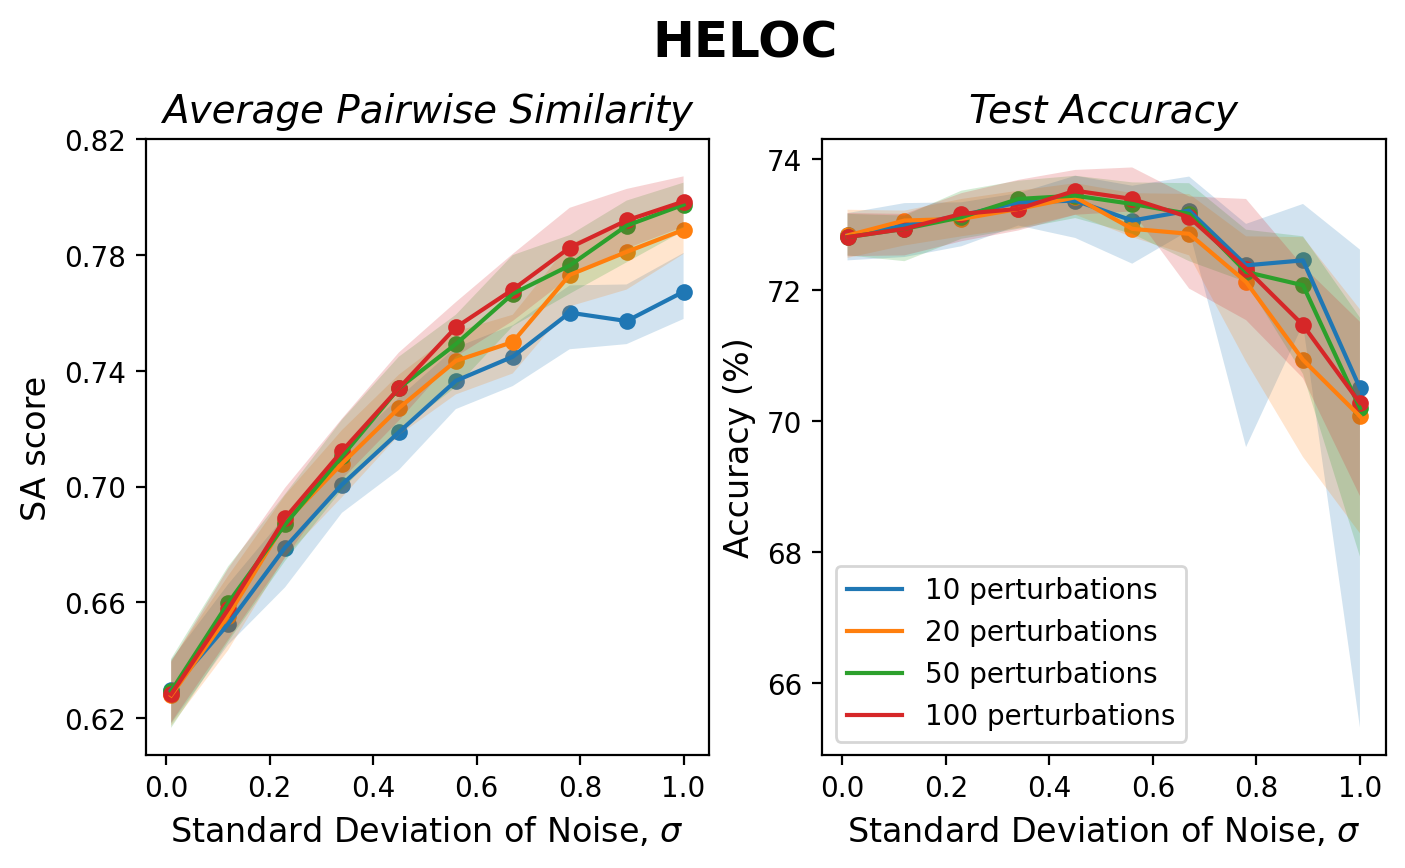
\includegraphics[width=0.325\textwidth]{figures/perturb_heloc_samples_bias.png}
    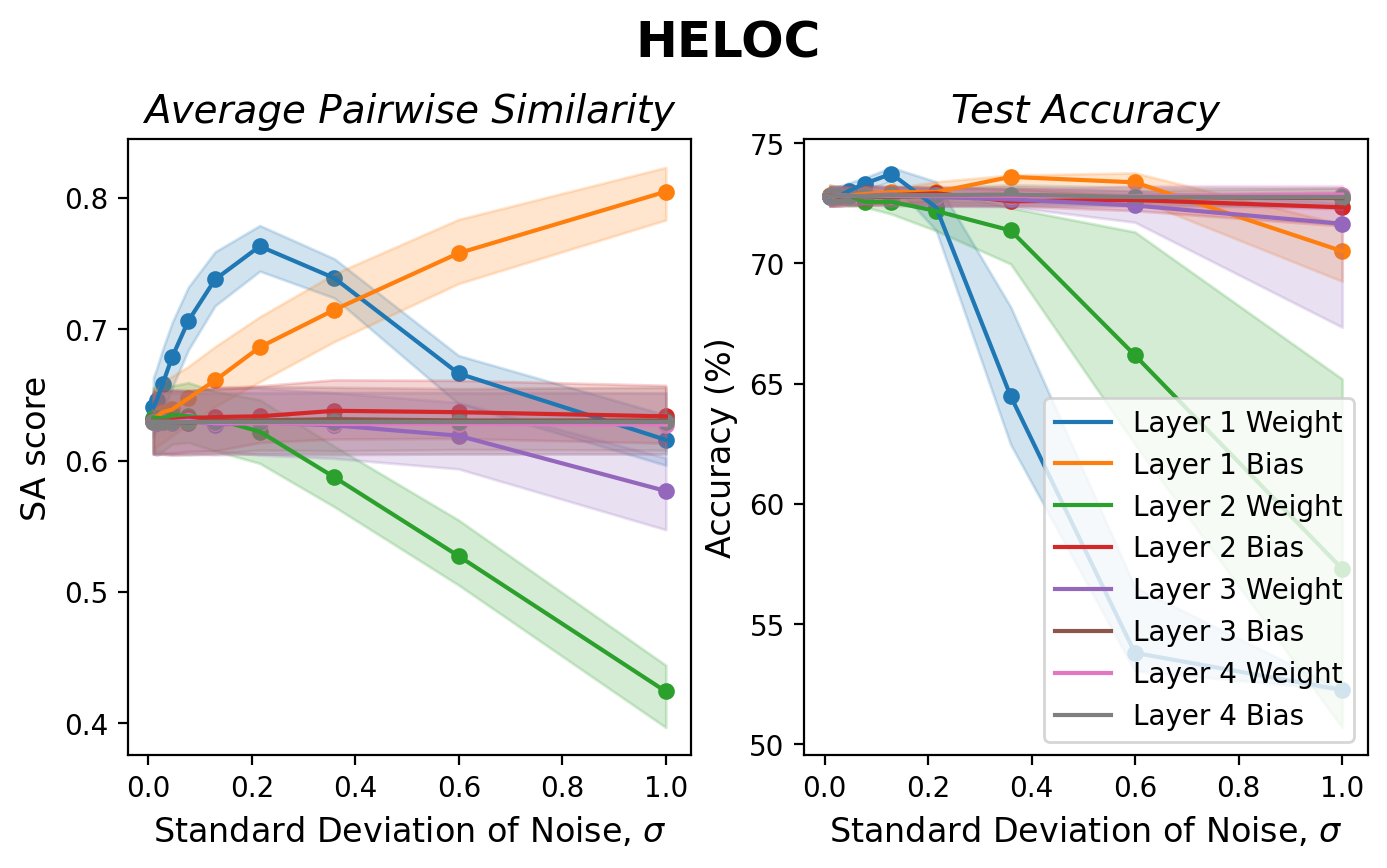
\includegraphics[width=0.325\textwidth]{figures/perturb_heloc_layers.png}
    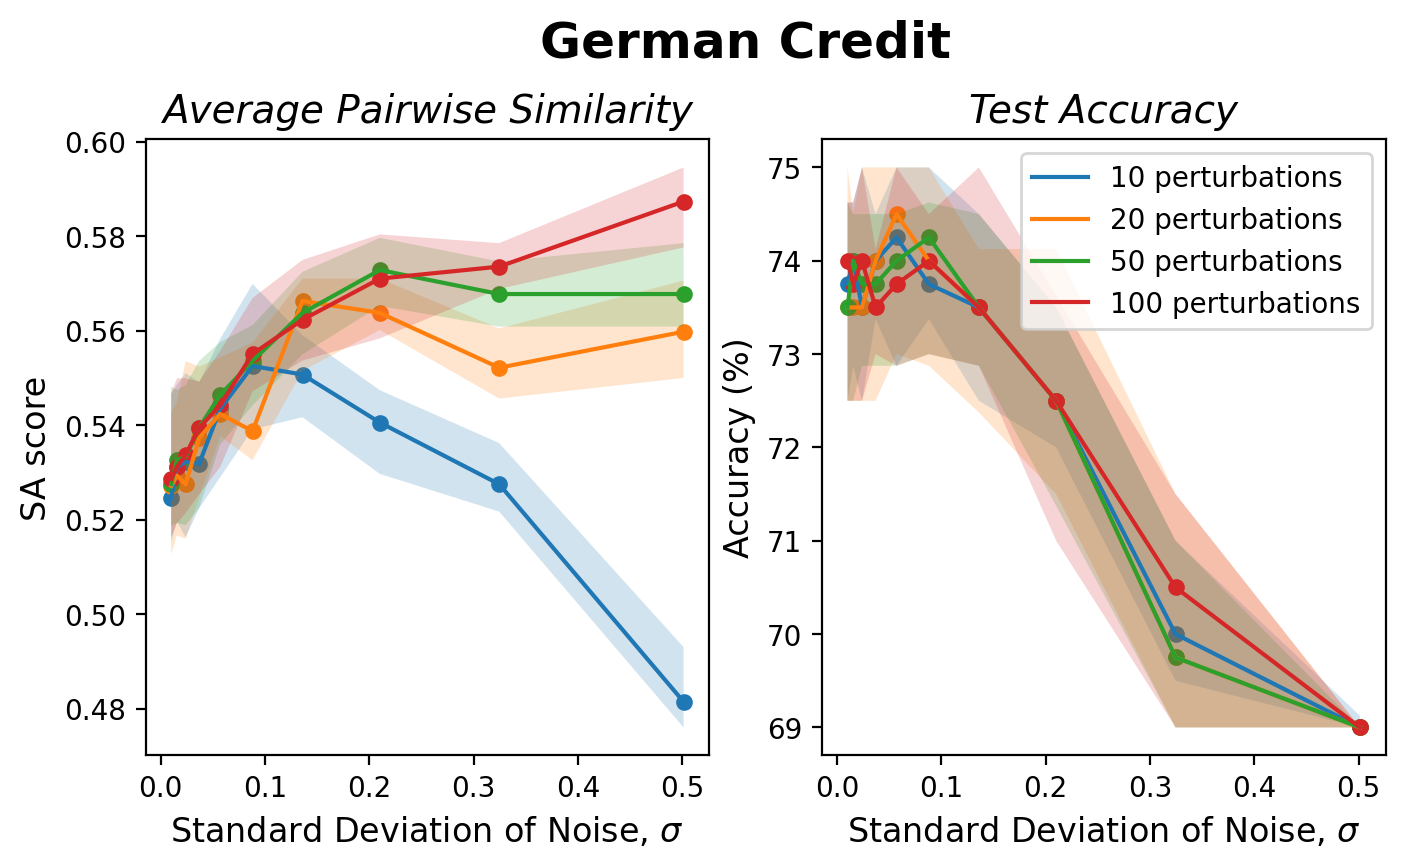
\includegraphics[width=0.325\textwidth]{figures/perturb_german_samples.png}
    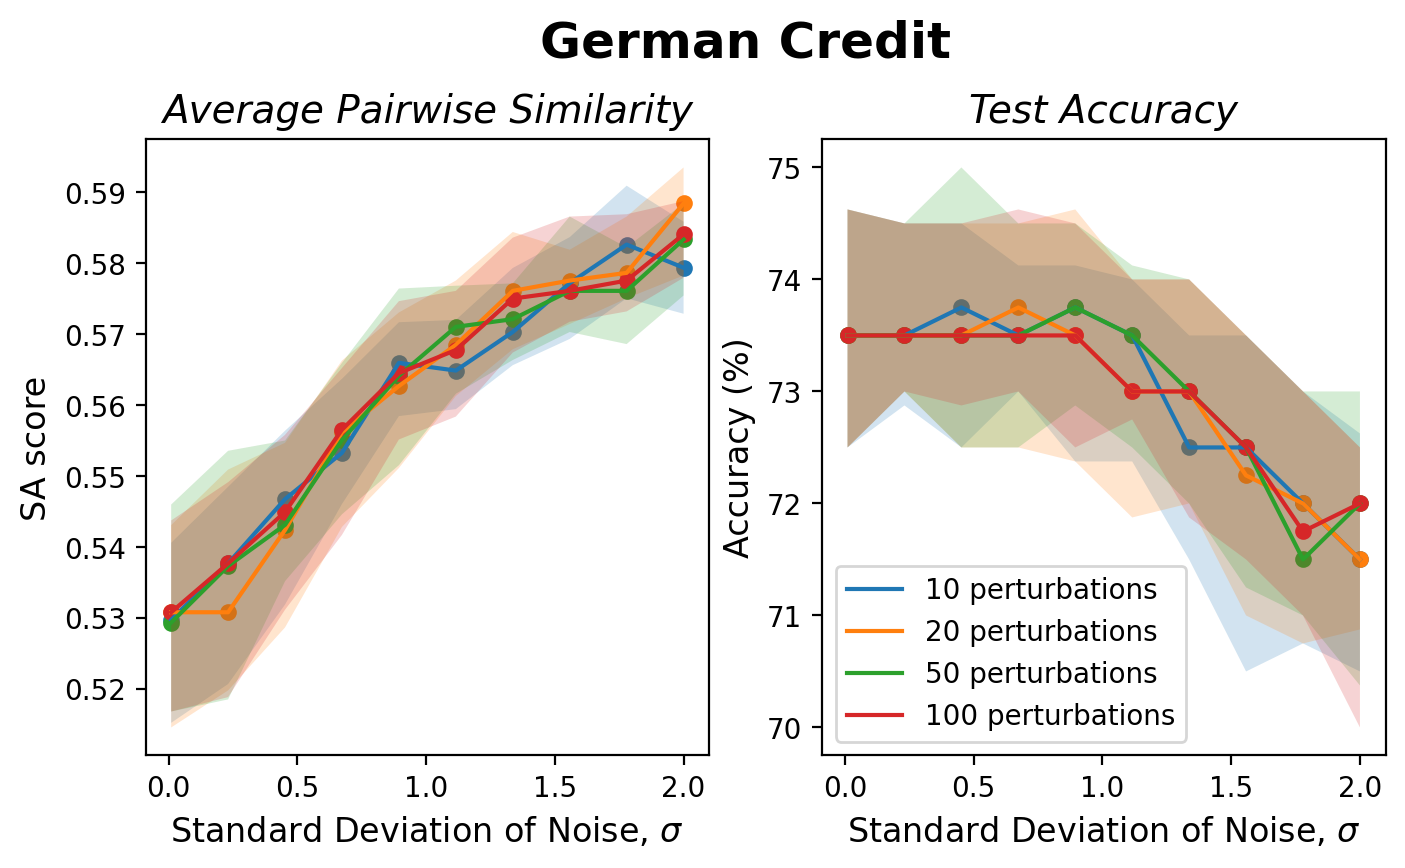
\includegraphics[width=0.325\textwidth]{figures/perturb_german_samples_bias.png}
    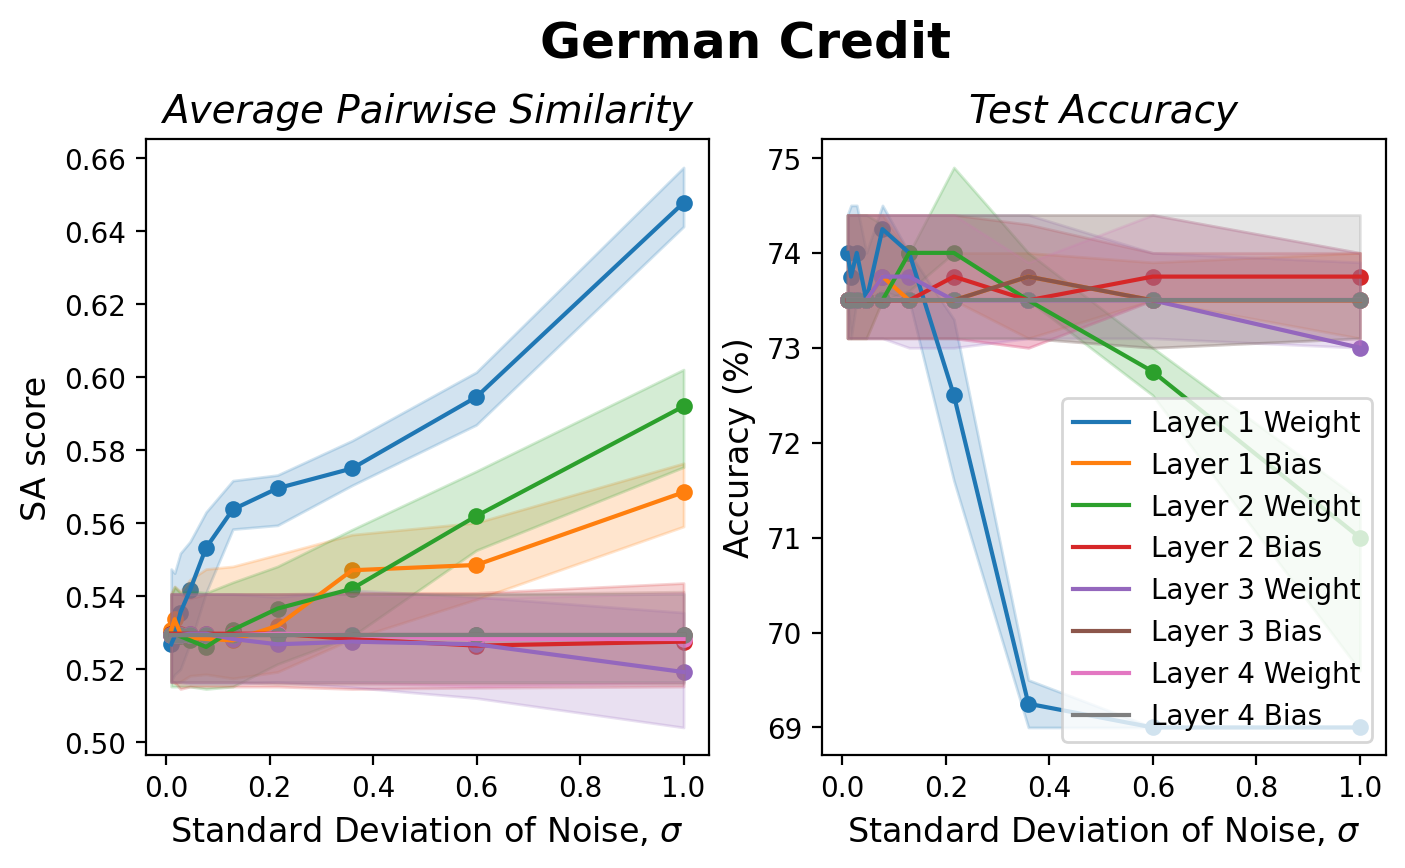
\includegraphics[width=0.325\textwidth]{figures/perturb_german_layers.png}
    \caption{\small Effect of $\sigma$ on top-k SA scores (for input gradients and $k=5$) and test accuracy on HELOC and German Credit datasets. \textbf{Left and Center:} perturbing the first layer weights, and the first layer biases, respectively. \textbf{Right:} perturbing layers individually 100 times each. Error bars represent the central decile of SA scores over 1000 individuals, and the interquartile range of accuracies over perturbed models.}
    \label{fig:perturb1}
\end{figure}

We present here full ablations across all datasets, to identify the optimal layer to perturb and the corresponding standard deviation $\sigma$ and number of perturbations, depicted in Figures~\ref{fig:perturb1} and~\ref{fig:perturb2}. As previously noted, the effects of random noise perturbations depend critically on the layer being perturbed. In most cases (bar German Credit or Adult Income), perturbing layers deeper than the first resulted in no increases in explanation similarity, and optimal gains were found by perturbing either the weights or biases of the first layer (i.e. connections between the input and the first hidden layer of size 128). We also trialled perturbing all layers cumulatively, or perturbing layers with noise proportional to the loss gradient of each weight, though could not identify superior results.

\begin{figure}[t]
    \centering
    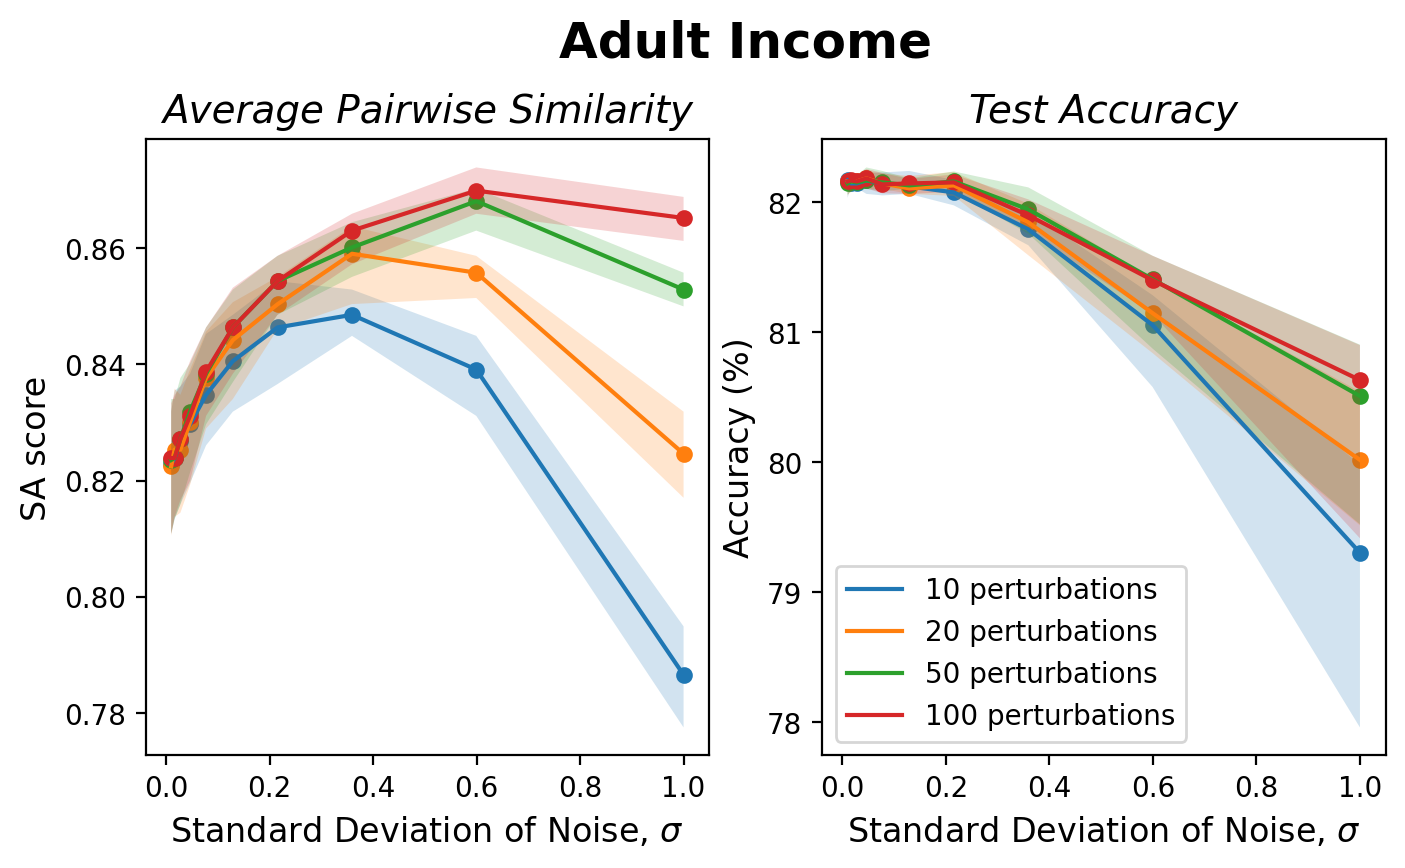
\includegraphics[width=0.325\textwidth]{figures/perturb_adult_samples.png}
    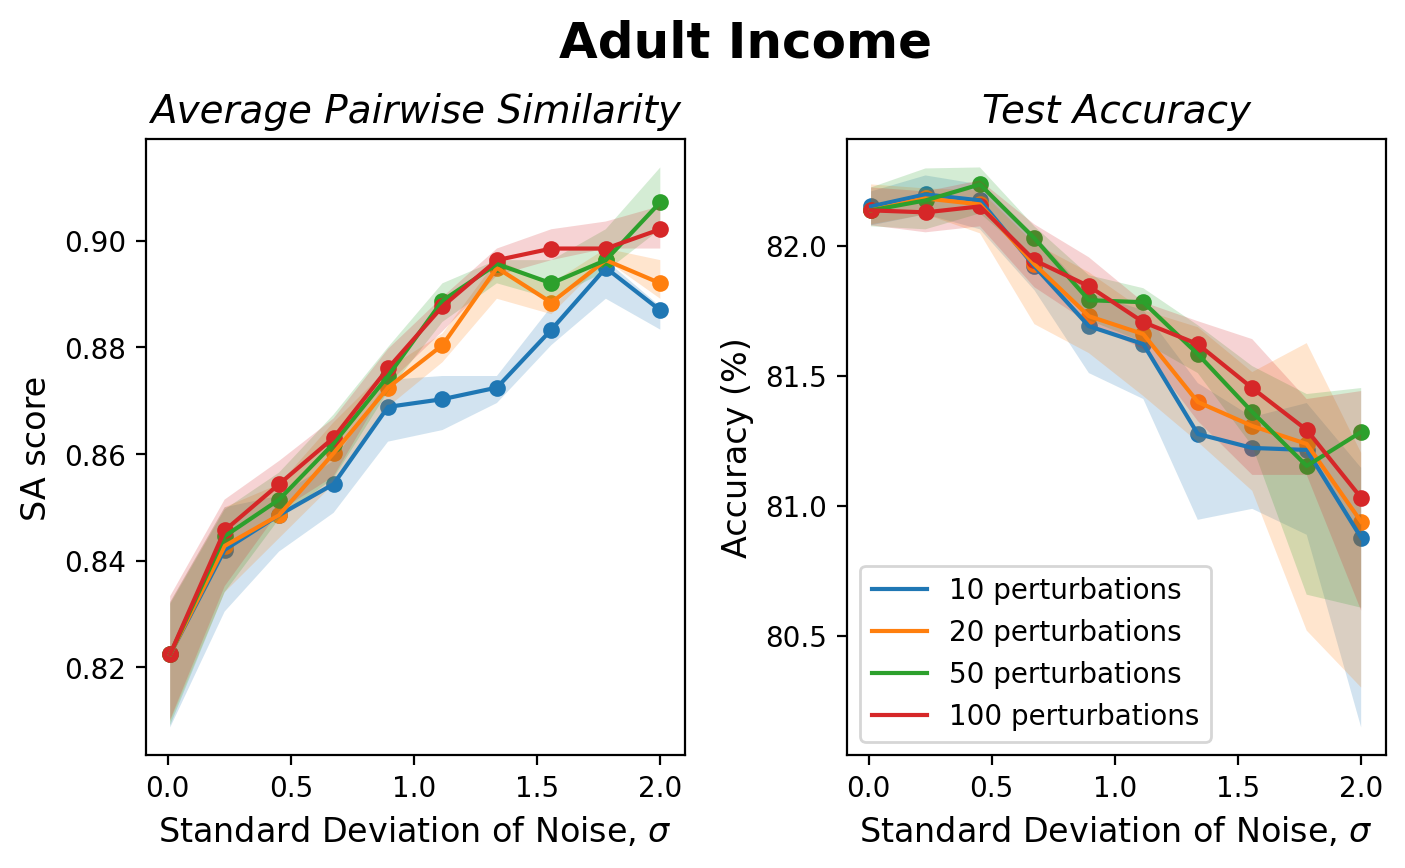
\includegraphics[width=0.325\textwidth]{figures/perturb_adult_samples_bias.png}
    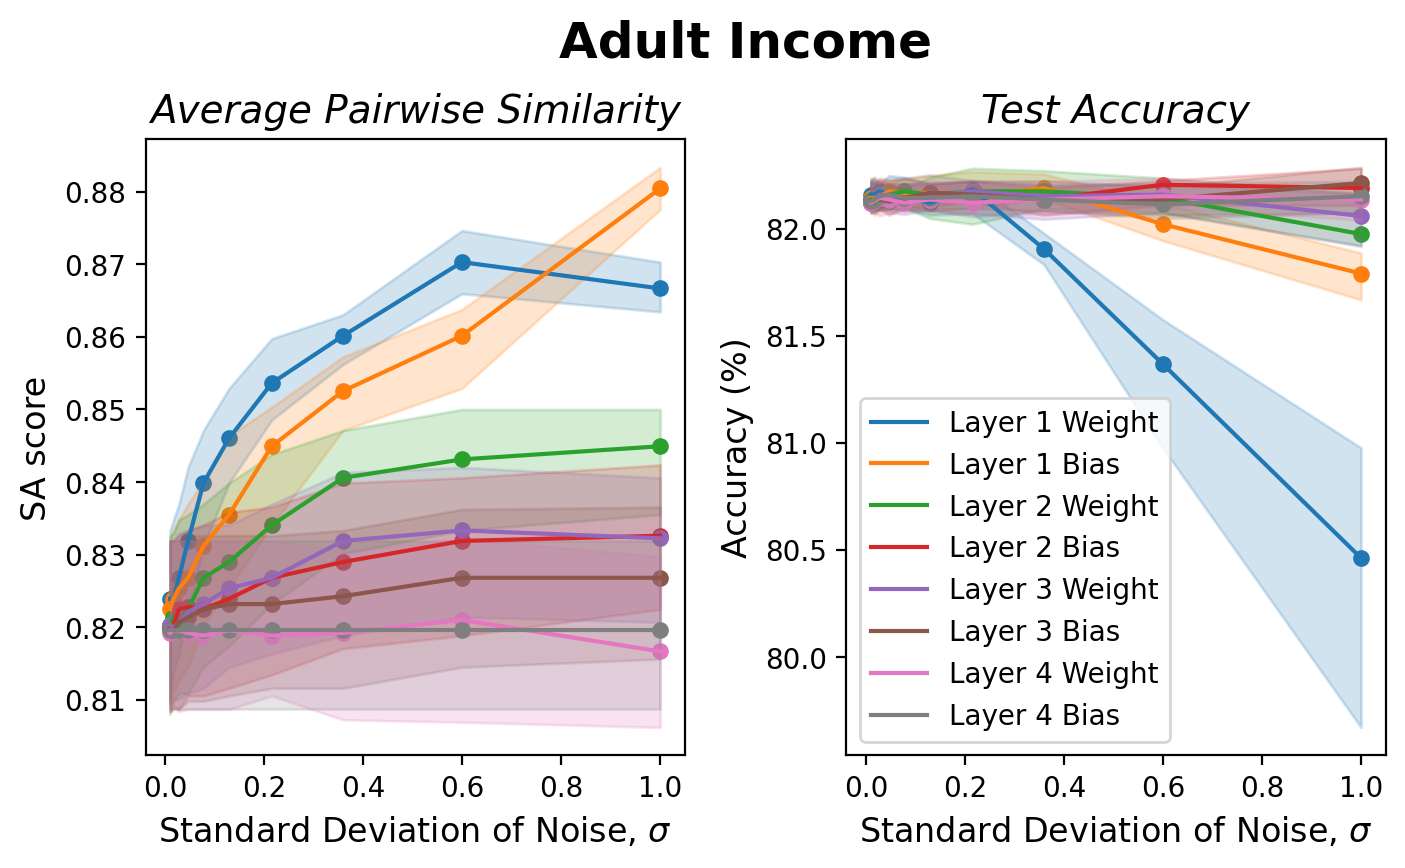
\includegraphics[width=0.325\textwidth]{figures/perturb_adult_layers.png}
    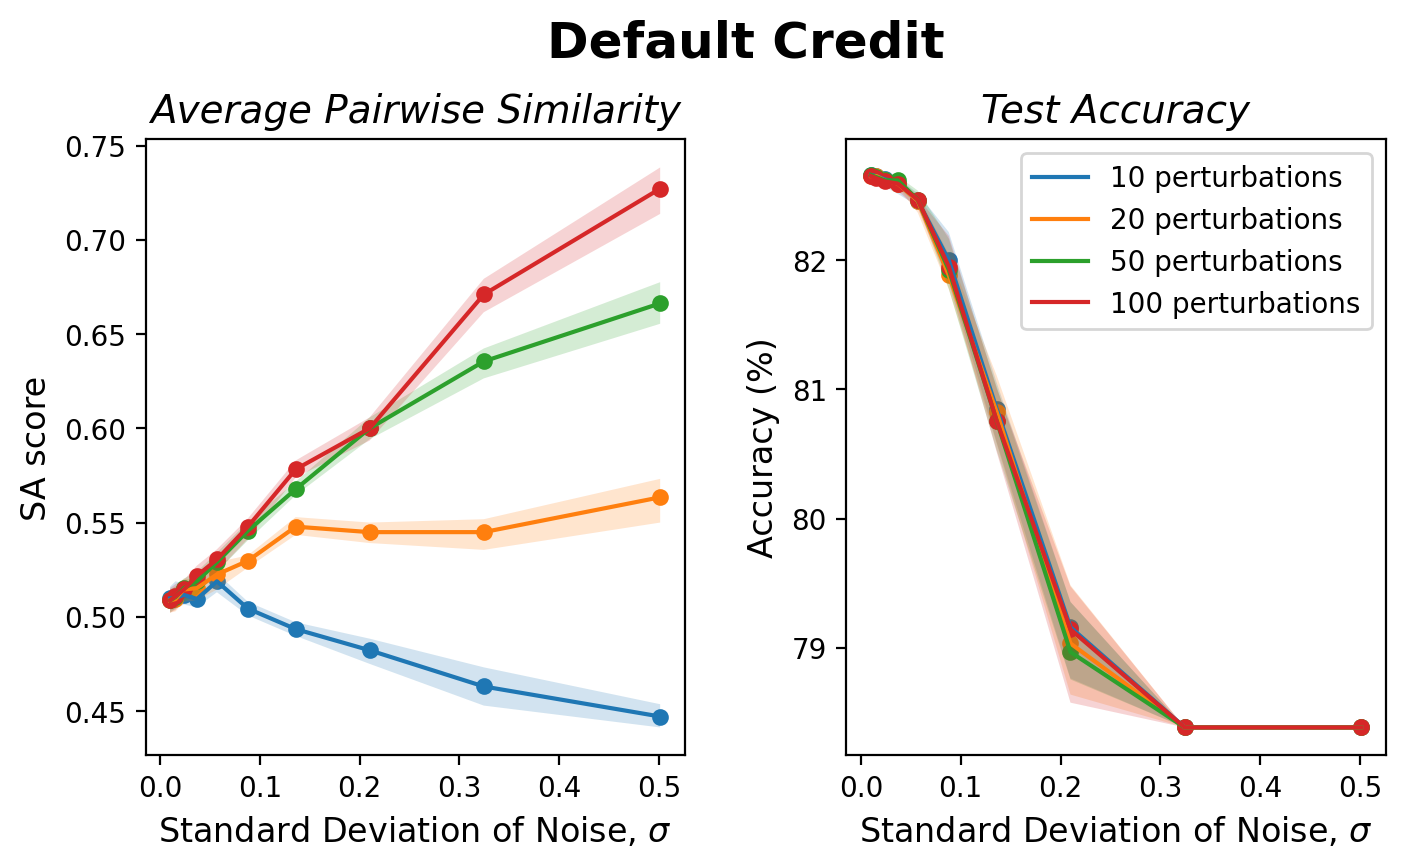
\includegraphics[width=0.325\textwidth]{figures/perturb_default_samples.png}
    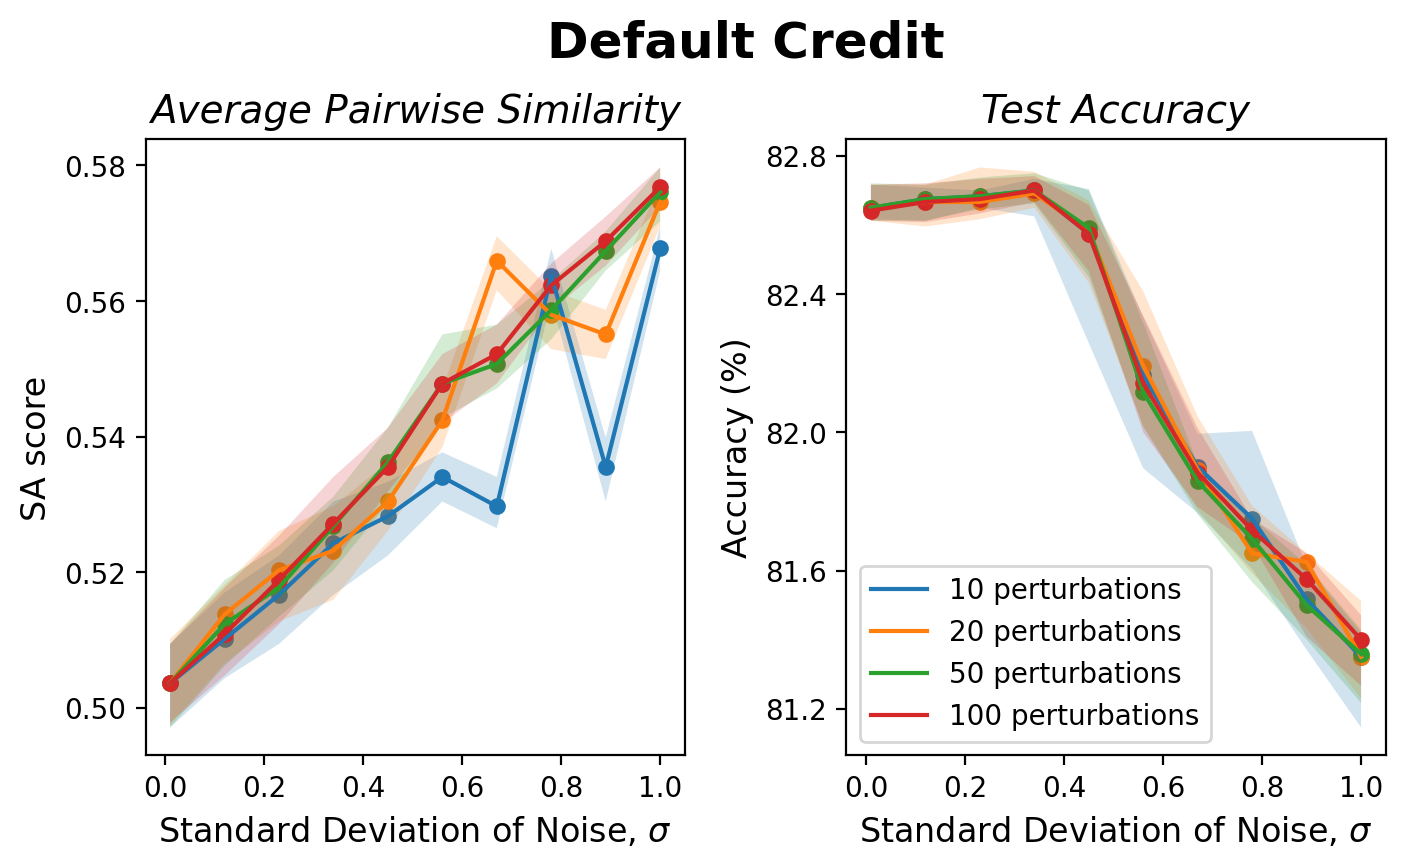
\includegraphics[width=0.325\textwidth]{figures/perturb_default_samples_bias.png}
    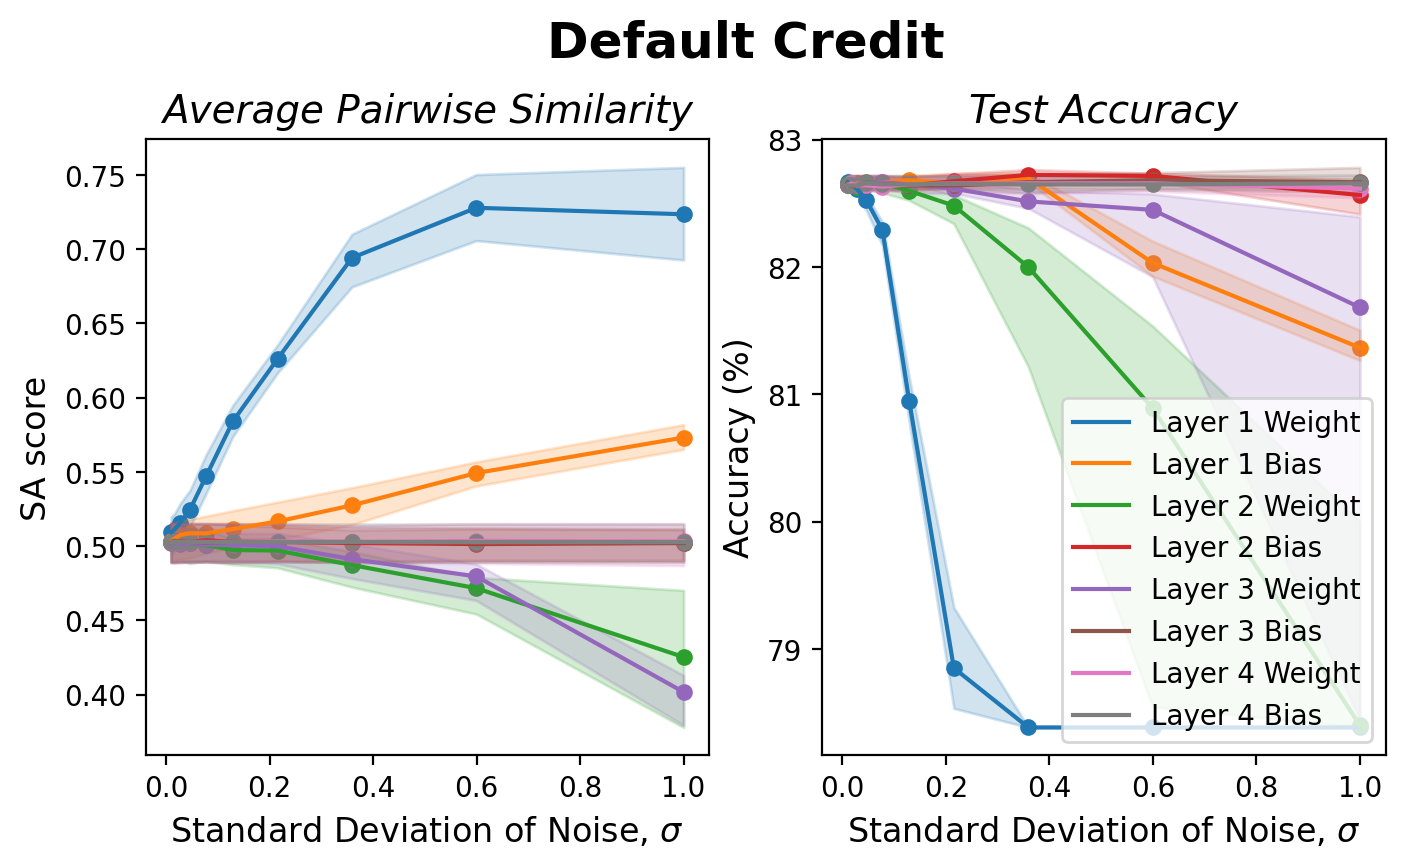
\includegraphics[width=0.325\textwidth]{figures/perturb_default_layers.png}
    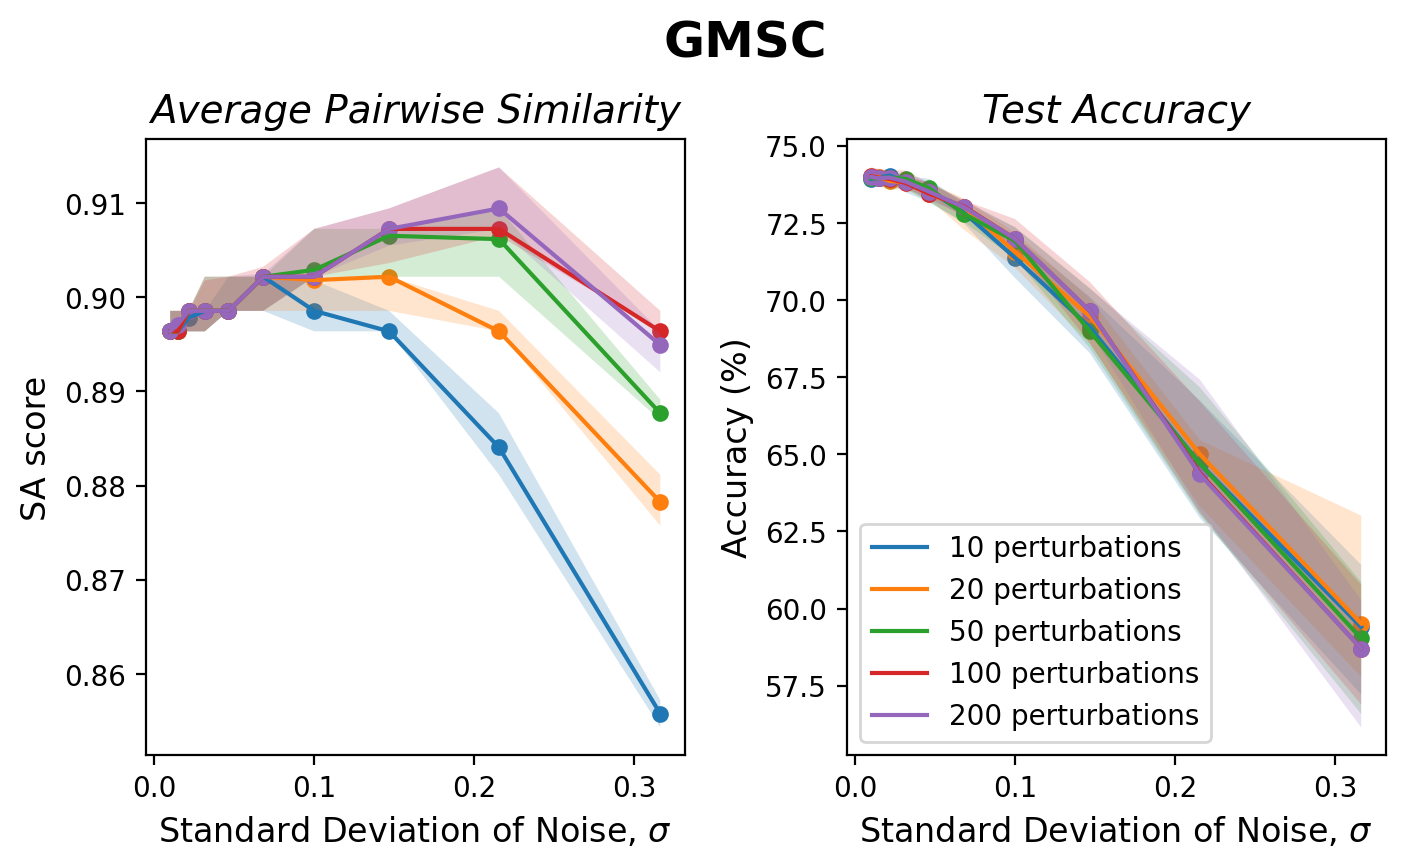
\includegraphics[width=0.325\textwidth]{figures/perturb_gmsc_samples.png}
    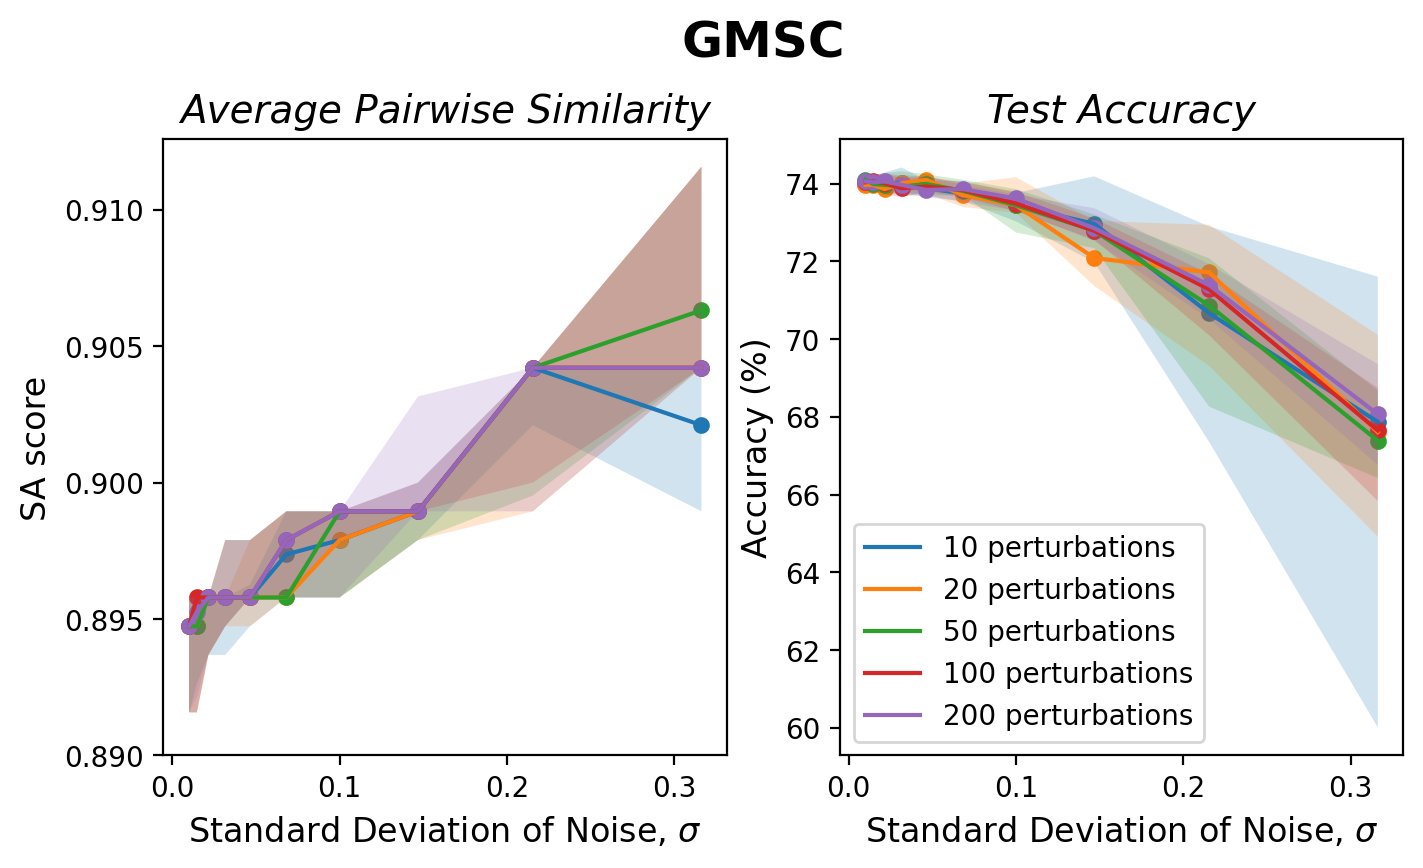
\includegraphics[width=0.325\textwidth]{figures/perturb_gmsc_samples_bias.png}
    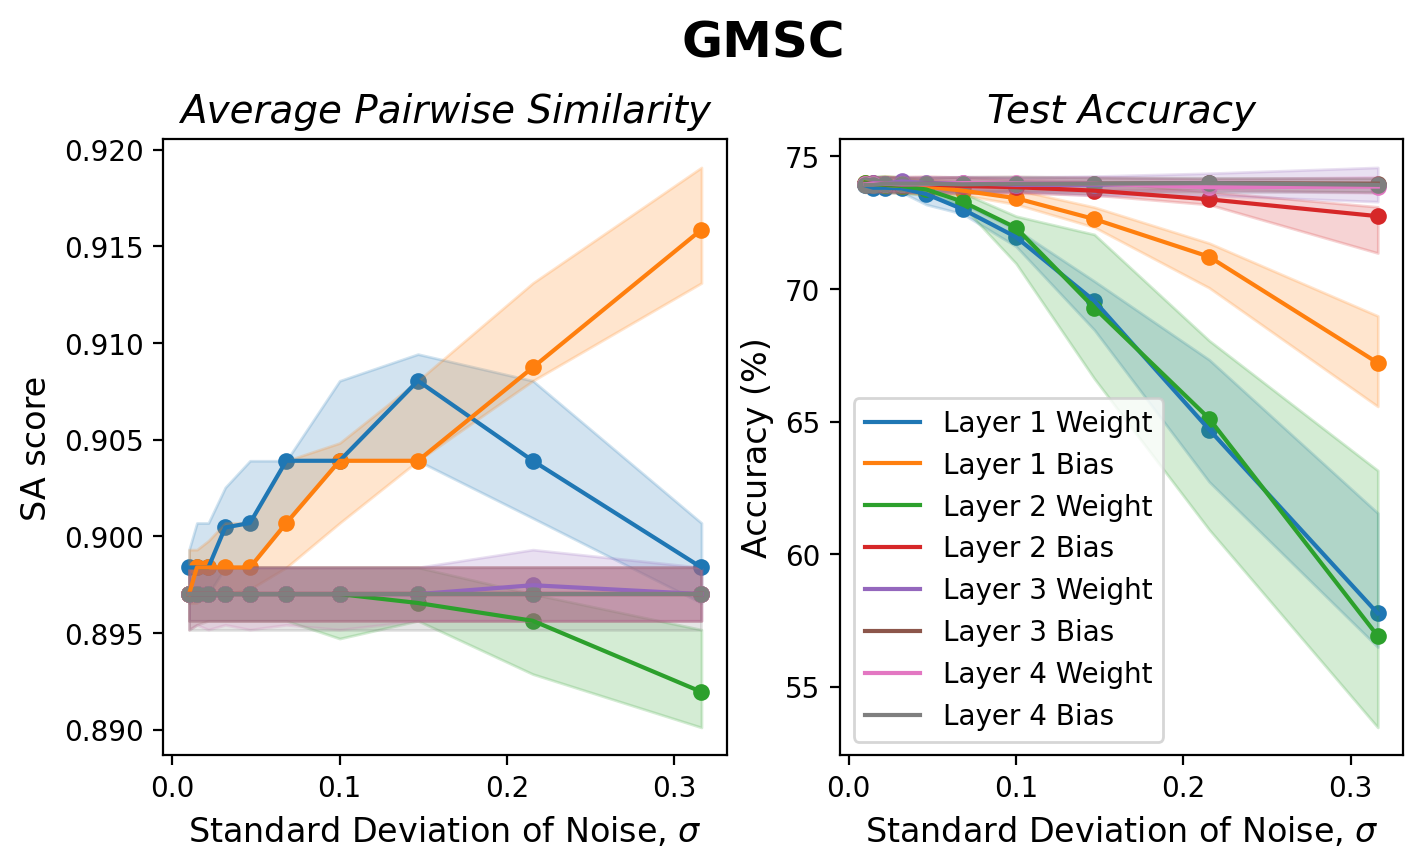
\includegraphics[width=0.325\textwidth]{figures/perturb_gmsc_layers.png}
    \caption{\small Effect of $\sigma$ on top-k SA scores (for input gradients and $k=5$) and test accuracy on Adult Income, Default Credit and GMSC datasets. \textbf{Left and Center:} perturbing the first layer weights, and the first layer biases, respectively. \textbf{Right:} perturbing layers individually 100 times each. Error bars represent the central decile of SA scores over 1000 individuals, and the interquartile range of accuracies over perturbed models.}
    \label{fig:perturb2}
\end{figure}

In our ensemble experiments, we perturb the bias of the first layer with standard deviations 0.05 and 0.5, for GMSC and Default Credit, respectively. We perturb the weights of the first layer with standard deviations 0.2, 0.2, and 0.3 for HELOC, German Credit and Adult Income, respectively. We use 50 perturbations in all cases, besides HELOC where we use 100 perturbations.

\section{Mode connectivity}
\label{app:mode}

\begin{figure}[b]
    \centering
    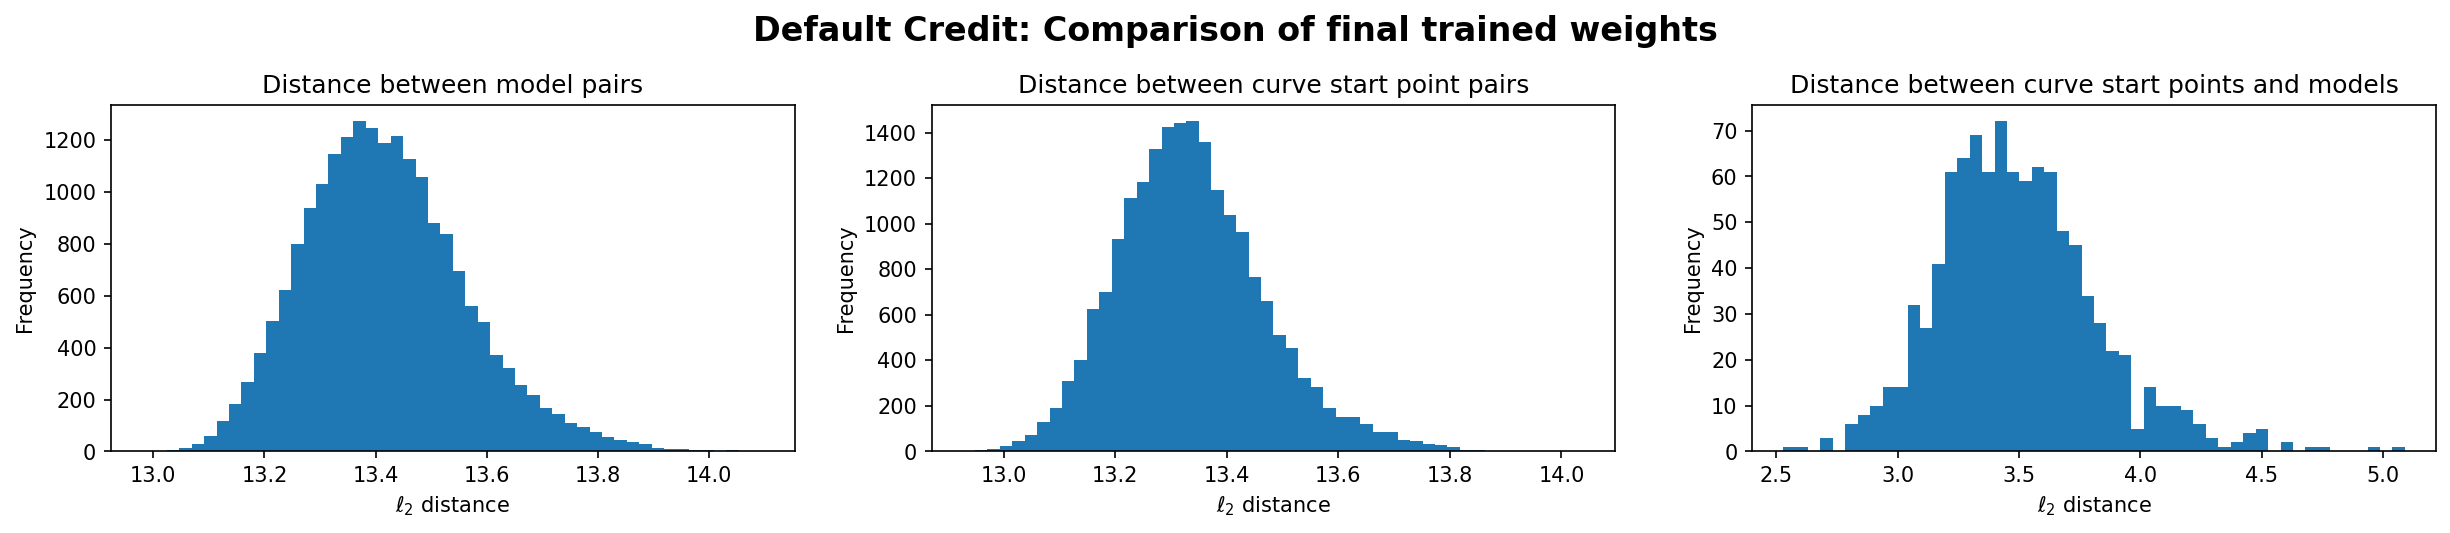
\includegraphics[width=\textwidth]{figures/modconn_approx.png}
    \caption{\small Mode connectivity approximation for Default Credit. Curve startpoints are similarly positioned in weight space to the original models, after training curves from scratch. \textbf{Left:} $\ell_2$ distance in weight space between model pairs in the underspecification set. \textbf{Center:} $\ell_2$ distance in weight space between curve \textit{startpoint} pairs. There is similar distance between pairs of curve startpoints after training curves, compared to between standard model pairs. \textbf{Right:} $\ell_2$ distance between trained curve startpoints and trained models is low.}
    \label{fig:modconn_approx}
\end{figure}

This section details our mode connectivity implementation. Given two models from the underspecification set, one can connect the two models in weight space via paths or near constant loss. We use the publicly available code from \citet{garipov2018} to do so. This takes two models as a fixed startpoint and endpoint for the curve. A linear path between the startpoint and endpoint is initialized, and a fixed number of bends lying along this path are backpropagated in order to minimize training loss of points sampled uniformally randomly along the curve.

While this method yielded improvements similar to those detailed in the paper, it introduces additional training costs, since one must effectively train new models (the bends along the curve). An alternate approach, described in the main text, is to initialize the curve with untrained start and end points, and train the curve from scratch. We trialled this as an effective approximation to mode connecting process. Specifically, the startpoint of one curve is initialized with the same random seed as used to train a given model from the underspecification set (endpoint is initialized randomly). The curve is then trained with the exact same hyperparameters as the original model was trained with. The only difference is that loss is sampled along the curve, rather than just at the startpoint. We demonstrate in Figure~\ref{fig:modconn_approx} how this resulted in the startpoint of the curve being trained to a similar position in weight space as the original model (i.e. $\ell_2$ distances are low on the right hand graph, while distances between pairs of curve startpoints after training is similar to distances between pairs of models after training).

Future work can consider optimizing the mode connectivity process, such that paths can be found with reduced computational cost. Multiple prior work have indicated that \textit{linear mode connectivity}, i.e. straight-line paths between models of near constant loss, can be achieved via permutation of the weights used \citep{ainsworth2023, singh2020, tatro2020}. It is worth noting that the focus of our investigation was to analyze how \textit{local}, \textit{global}, or their \textit{combined} explorations of the loss landscape could promote explanation alignment after ensembling. The exact mechanisms used to explore the loss landscape, and their computational efficiencies, should build on related advancements, and is a ripe area for future work.

\section{Comparison of ensemble techniques}
\label{app:experiments}

This Appendix displays full results, similar to those in Figure~\ref{fig:ensembles}, but across all similarity metrics and explanation techniques. Recall that for the CDC metric, we aim to stress test our ensembling techniques by assessing top-$d$ similarity, where $d$ is the dimensionality of the data. This means that a score of 1 is returned only if the signs of all features match between two ensembles. For any particular number of pre-trained models, 50 ensembles are constructed, and for each individual in the test set, 

\begin{figure}[hb]
    \centering
    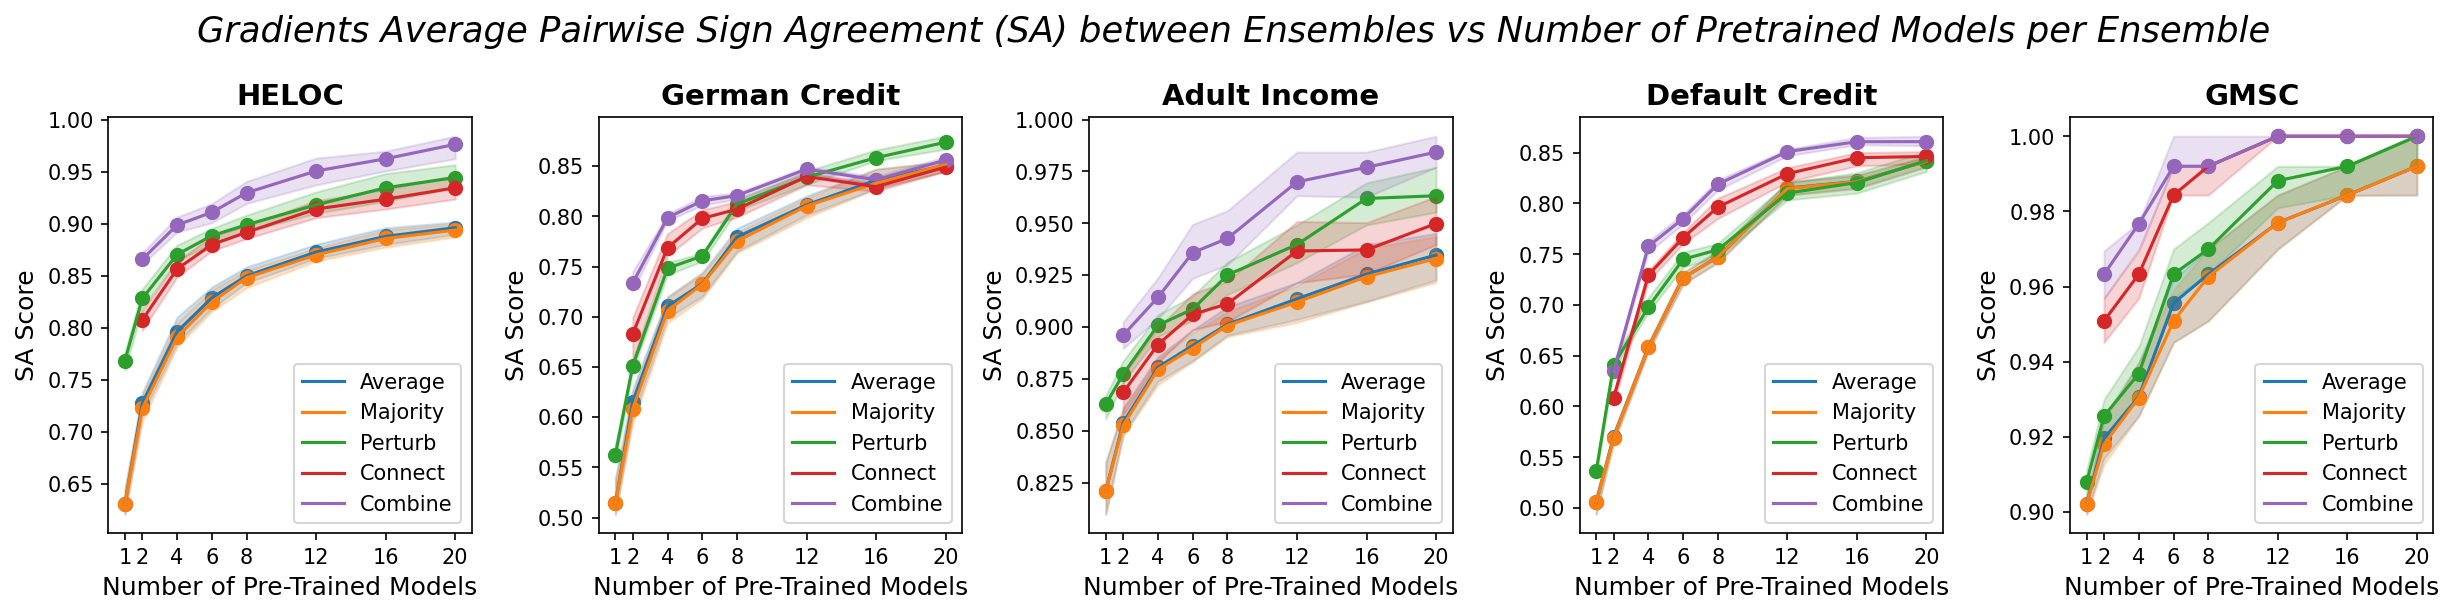
\includegraphics[width=0.99\textwidth]{figures/sa_top5_gradients.png}
    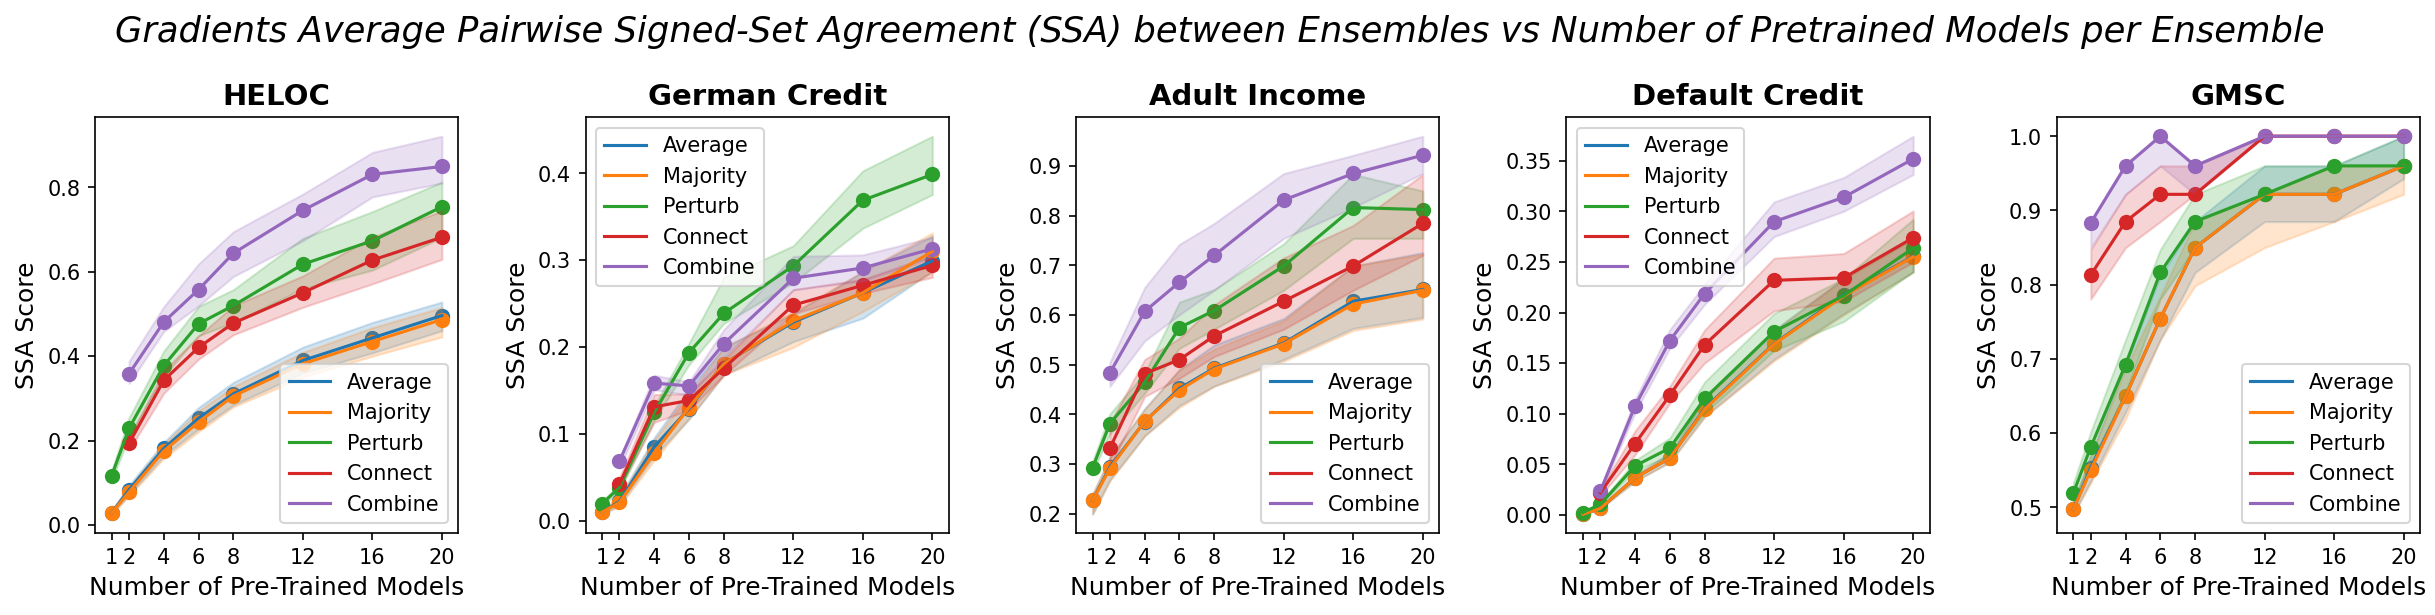
\includegraphics[width=0.99\textwidth]{figures/ssa_top5_gradients.png}
    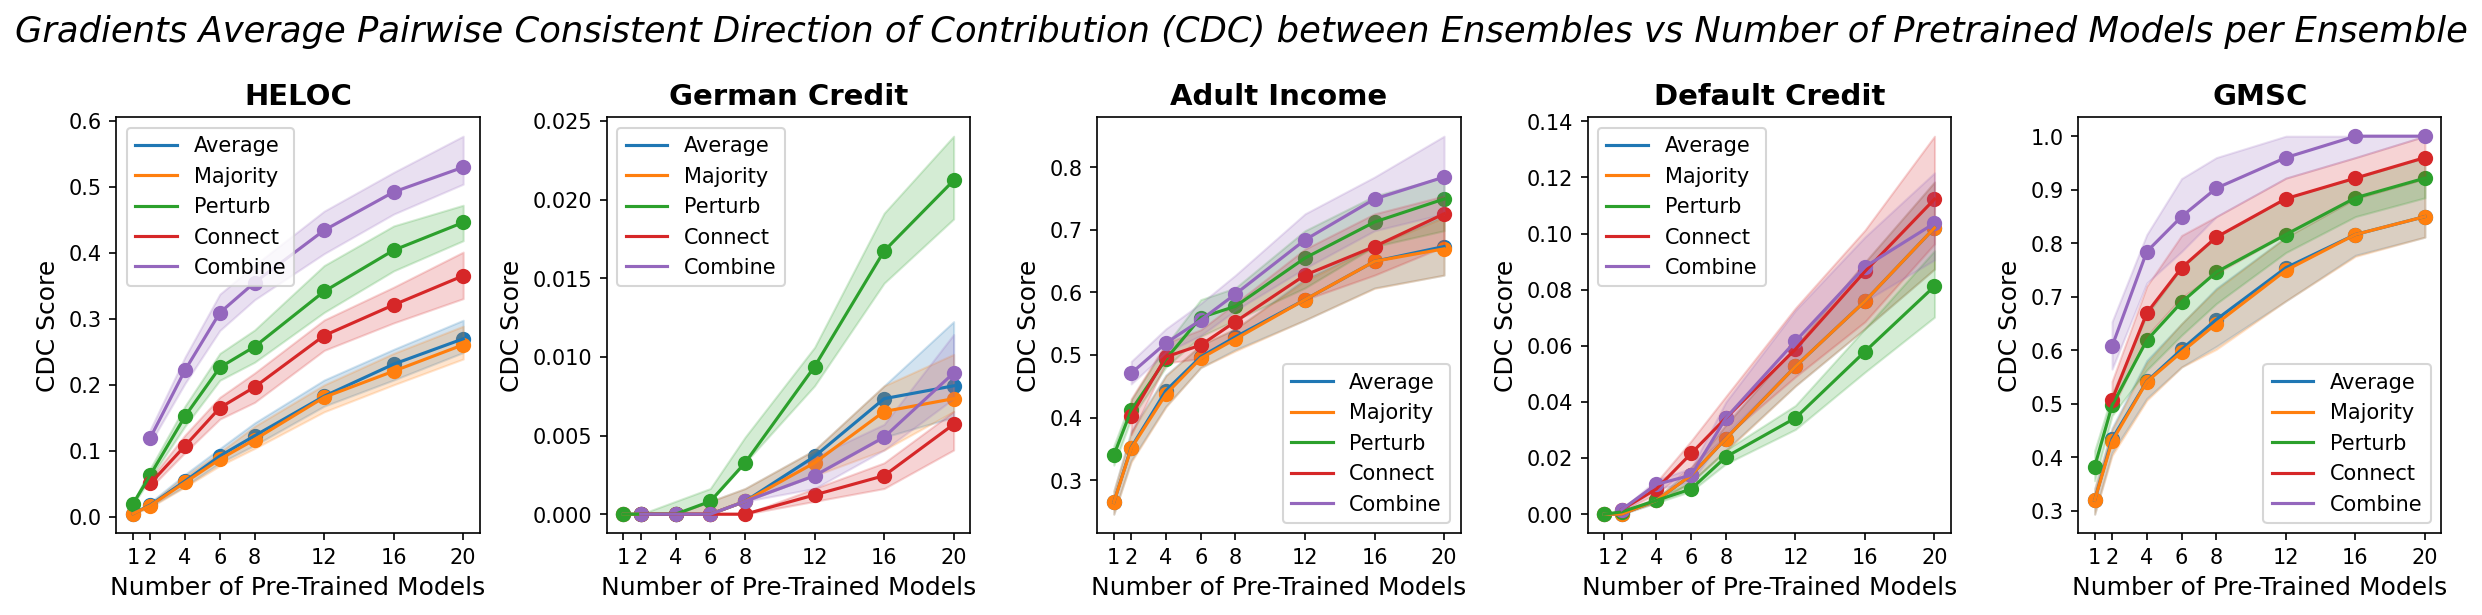
\includegraphics[width=0.99\textwidth]{figures/cdc_topd_gradients.png}
    \caption{\small Effectiveness of ensemble strategies in stabilizing explanations across all datasets (top-5 SA, top-5 SSA, and top-$d$ CDC scores for \textbf{input gradients}). \textit{Average} and \textit{Majority} denote vanilla ensembles, while \textit{Perturb}, \textit{Connect}, and \textit{Combine} denote weight perturbation, mode connectivity, and their combination respectively.}
    \label{fig:ensembles_all}
\end{figure}
average similarities are computed across all $\binom{50}{2}$ = 1225 unique pairs. The median individual similarity is plotted, and error bars indicated the central decile of individuals.

\paragraph{Effects of ensembling on Saliency} Figure~\ref{fig:ensembles_all} details full results for input gradients i.e. Saliency. The central row is depicted in the main text (Figure~\ref{fig:ensembles}). Observe similar trends between SA scores (top row) and SSA scores (central row), as the latter is a stricter (binary) version of the former. Top-$d$ CDC comparisons demonstrate similar trends. For instance, to exceed 80\% similarity on the GMSC dataset, standard ensembling (blue and orange) requires around 20 pre-trained models, while the combined exploration of mode connectivity alongside local perturbations (purple) requires 4 pre-trained models.

\paragraph{Effects of ensembling on Smoothgrad} Figure~\ref{fig:ensembles_all_sg} details full results for Smoothgrad, where we use 50 perturbations on the input with standard deviation 0.1. Note that this explanation technique generally improves explanation similarity slightly for standard ensembles (blue and orange), e.g., for 20 pre-trained models, median SSA scores on Adult Income increase from 60\% in Figure~\ref{fig:ensembles_all} to 70\% in Figure~\ref{fig:ensembles_all_sg}. However, our findings suggest that Smoothgrad does not provide significant smoothing benefits for explanation alignment beyond our ensemble techniques. Specifically, for the same comparison of median SSA scores on Adult Income, when considering 20 pre-trained models, both Smoothgrad and saliency techniques achieve approximately 90\% explanation alignment using the combined approach, while local perturbations or mode connectivity yield around 80\% alignment. Furthermore, while Smoothgrad provides an explanation for a smoothed approximation of a potentially noisy decision boundary, ensemble approaches smooth both the explanation and the model's decision region.

\begin{figure}[bh]
    \centering
    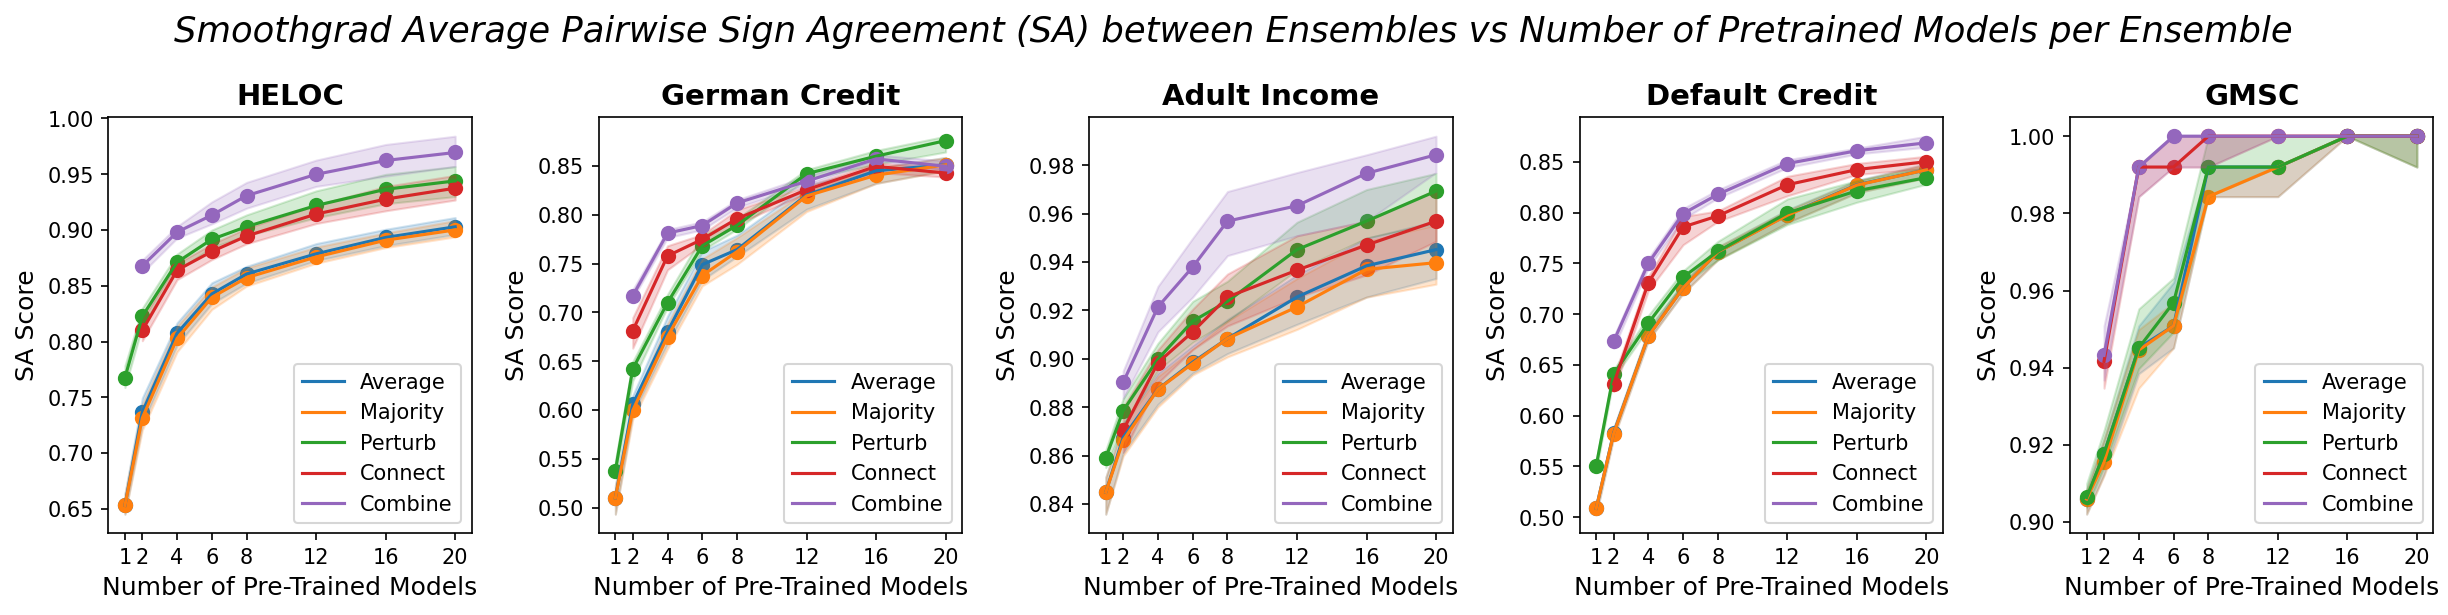
\includegraphics[width=0.99\textwidth]{figures/sa_top5_smoothgrad.png}
    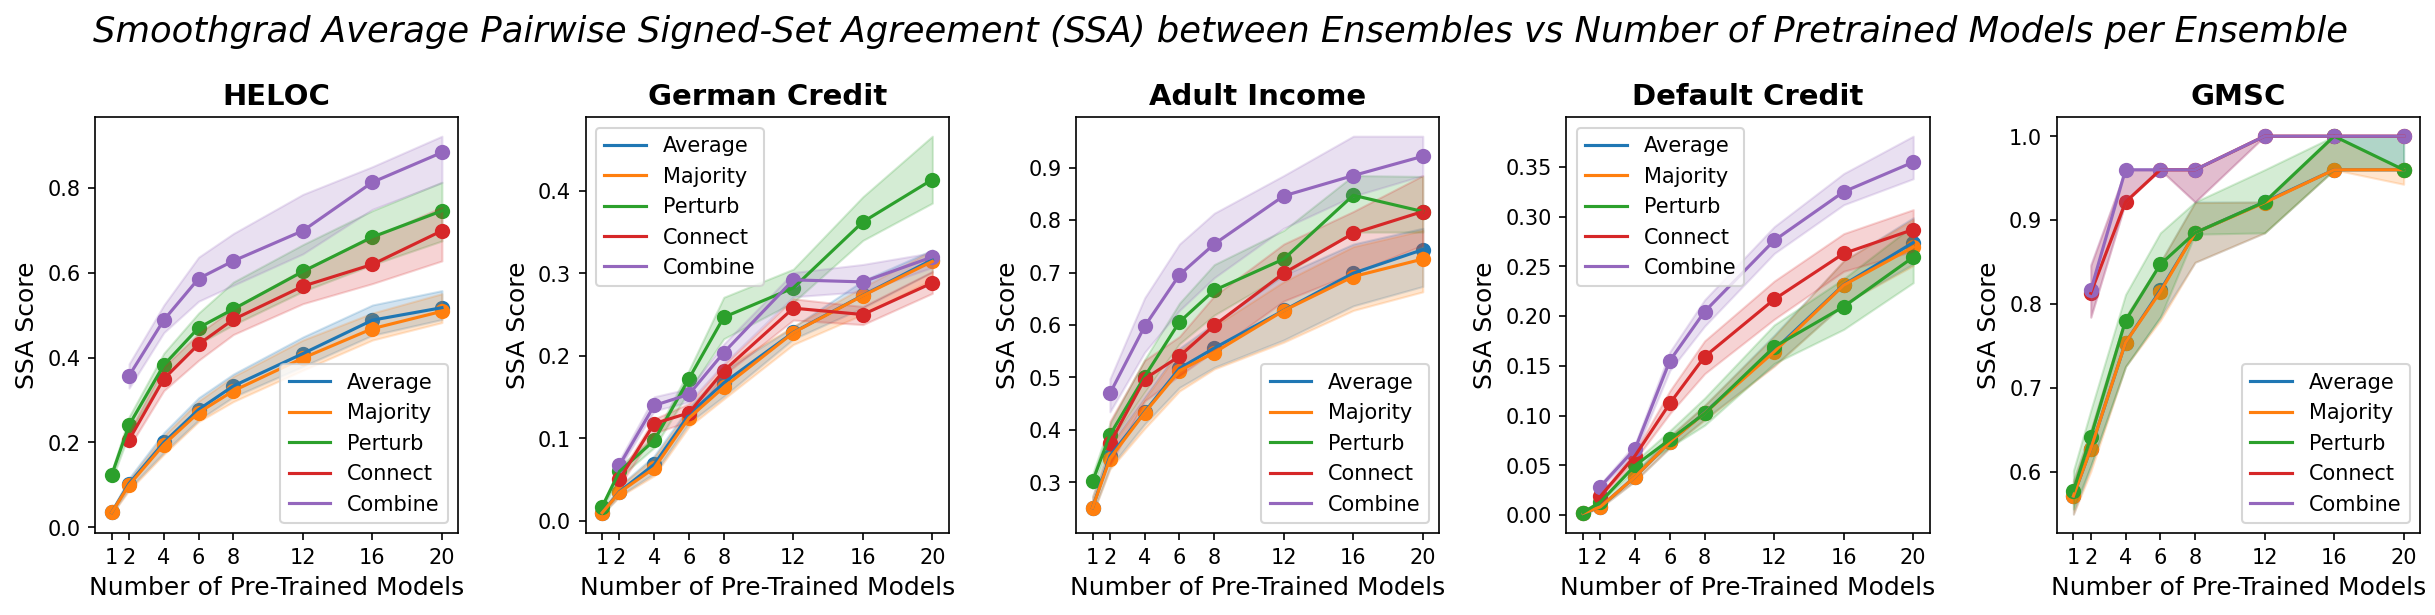
\includegraphics[width=0.99\textwidth]{figures/ssa_top5_smoothgrad.png}
    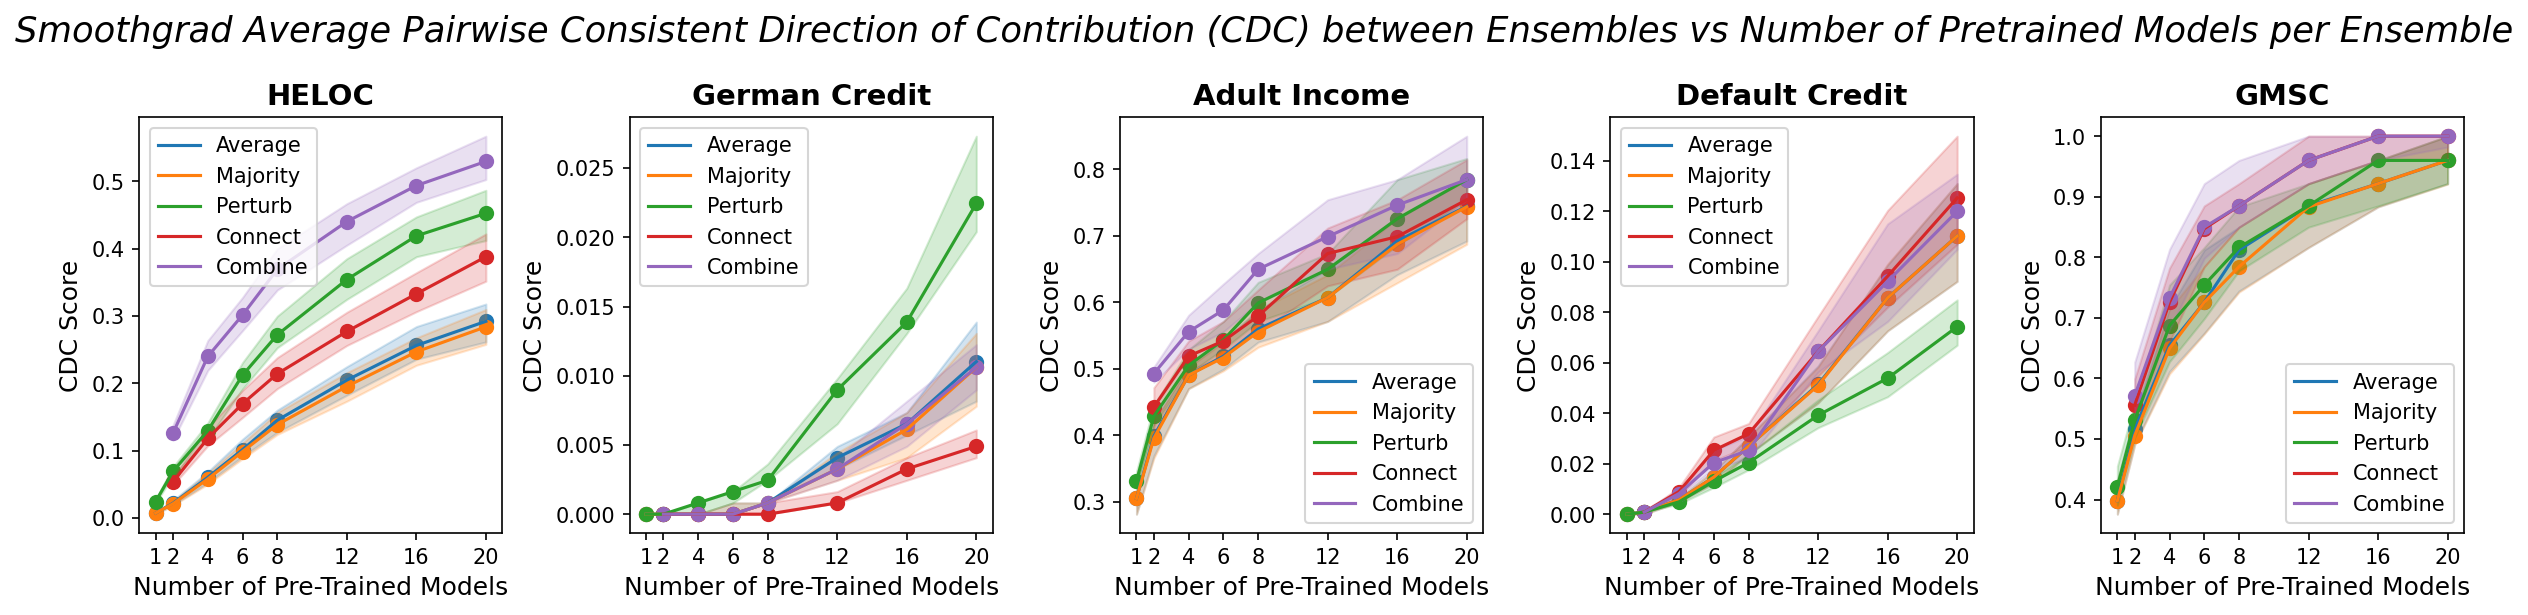
\includegraphics[width=0.99\textwidth]{figures/cdc_topd_smoothgrad.png}
    \caption{\small Effectiveness of ensemble strategies in stabilizing explanations across all datasets (top-5 SA, top-5 SSA, and top-$d$ CDC scores for \textbf{Smoothgrad}). \textit{Average} and \textit{Majority} denote vanilla ensembles, while \textit{Perturb}, \textit{Connect}, and \textit{Combine} denote weight perturbation, mode connectivity, and their combination respectively.}
    \label{fig:ensembles_all_sg}
\end{figure}

\paragraph{Effects of ensembling on DeepSHAP} Figure~\ref{fig:ensembles_all_shap} details full results for DeepSHAP, an approximation to SHAP that leverages knowledge from the neural network directly. Note first that results may be slightly noisier, given the computational restriction of using this method (the first 100 test points in each datasets are evaluated, rather than the first 1000 as in other methods). In spite of this, the various ensembling techniques proposed, for a given number of pre-trained models, tend to yield benefits similar to previously e.g. HELOC trends are largely similar after accounting for noise fluctuations. SA and SSA scores for DeepSHAP tended to have higher baseline similarity scores (i.e. between single models) compared to Saliency and Smoothgrad. We see notable improvements for the mode connected/combined explorations for Adult Income, Default Credit and GMSC. However, we also observe the one instance where mode connectivity was inferior to standard ensembling, in German Credit. While this was overcome through the combined technique of sampling along connected modes and further perturbing each of the samples (purple), and secondly that local weight perturbation alone improved performance, this emphasizes the unpredictable nature of particular explanation techniques, and warrants future research. A \textit{sufficiently large} number of pre-trained models may eliminate explanation multiplicity, and so the focus of future work should be on exploiting further the properties of the loss landscape to optimize the local and global searches for ensemble members.

\begin{figure}[ht]
    \centering
    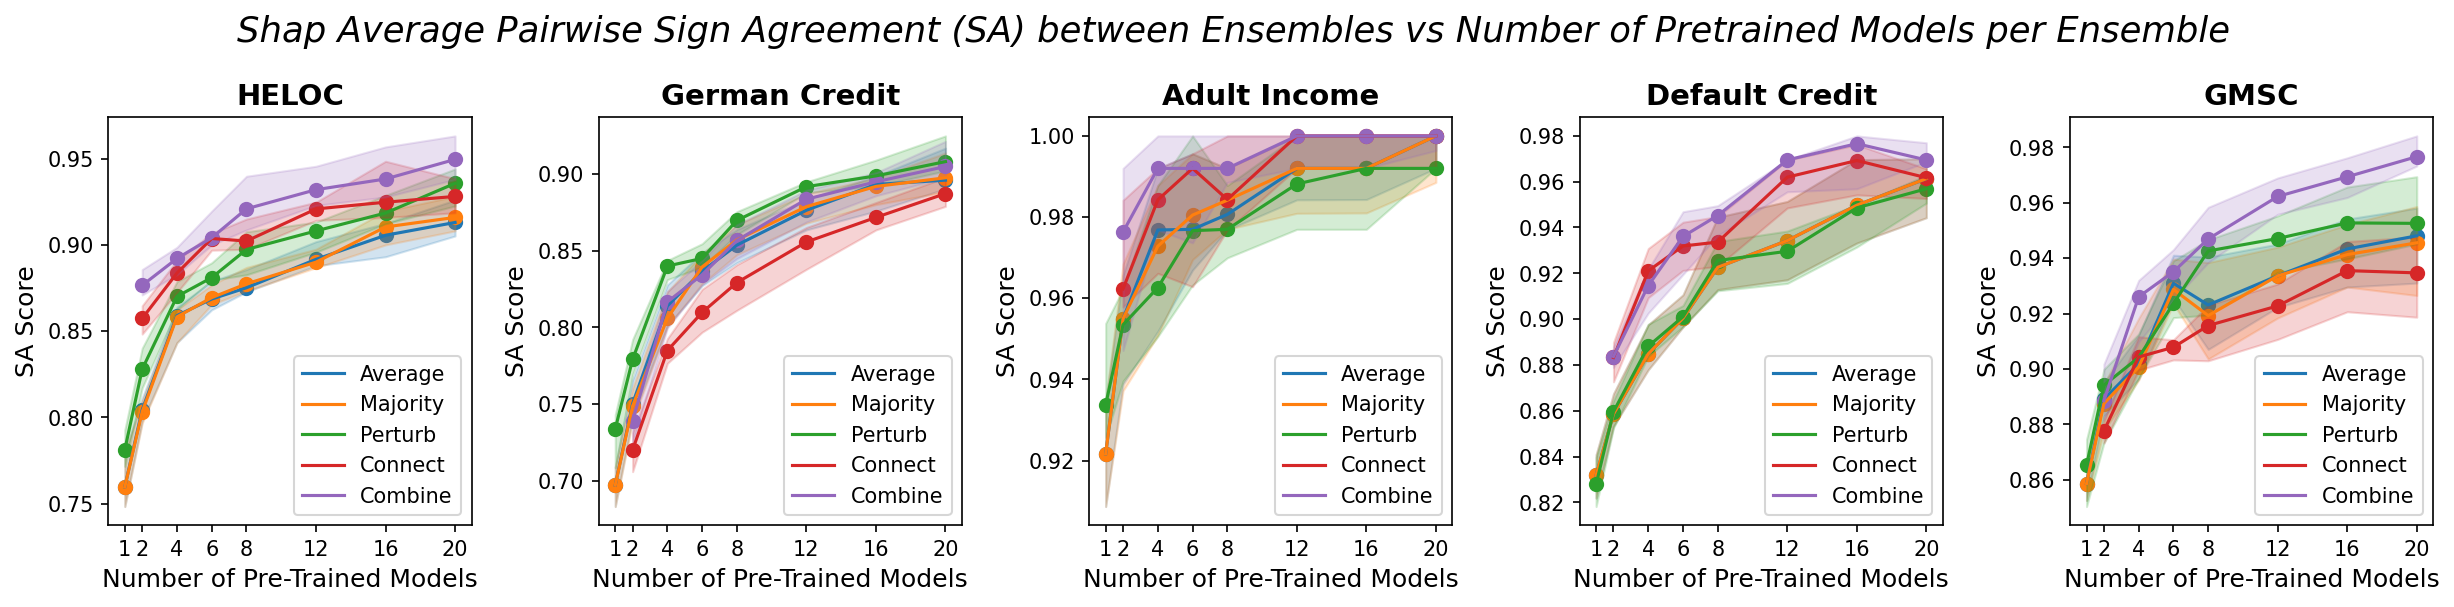
\includegraphics[width=0.99\textwidth]{figures/sa_top5_shap.png}
    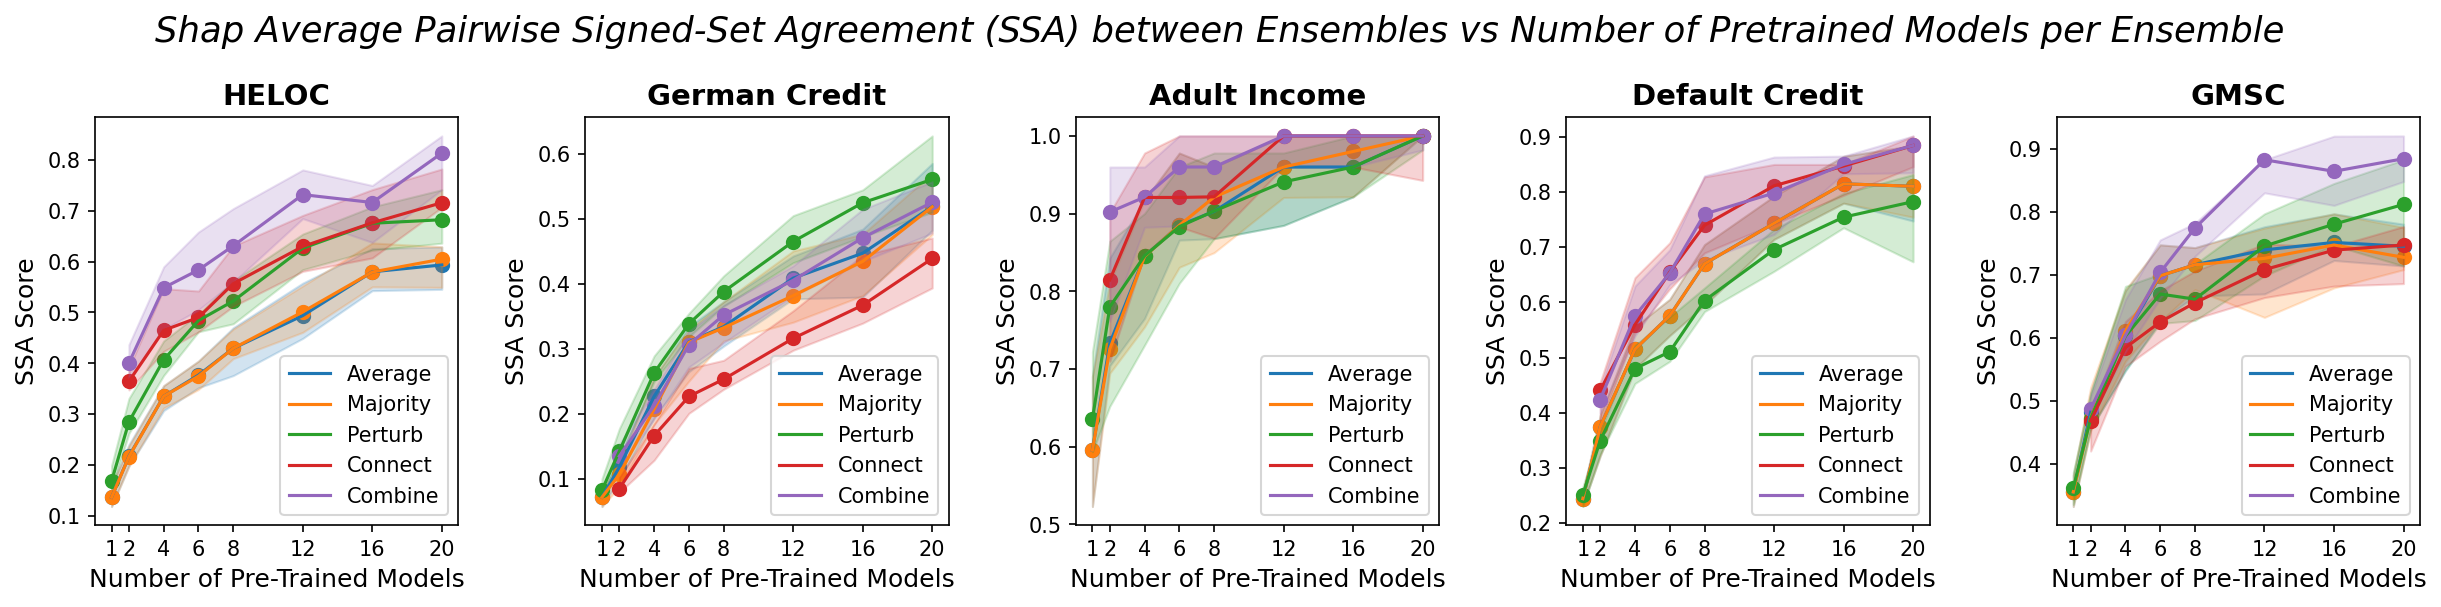
\includegraphics[width=0.99\textwidth]{figures/ssa_top5_shap.png}
    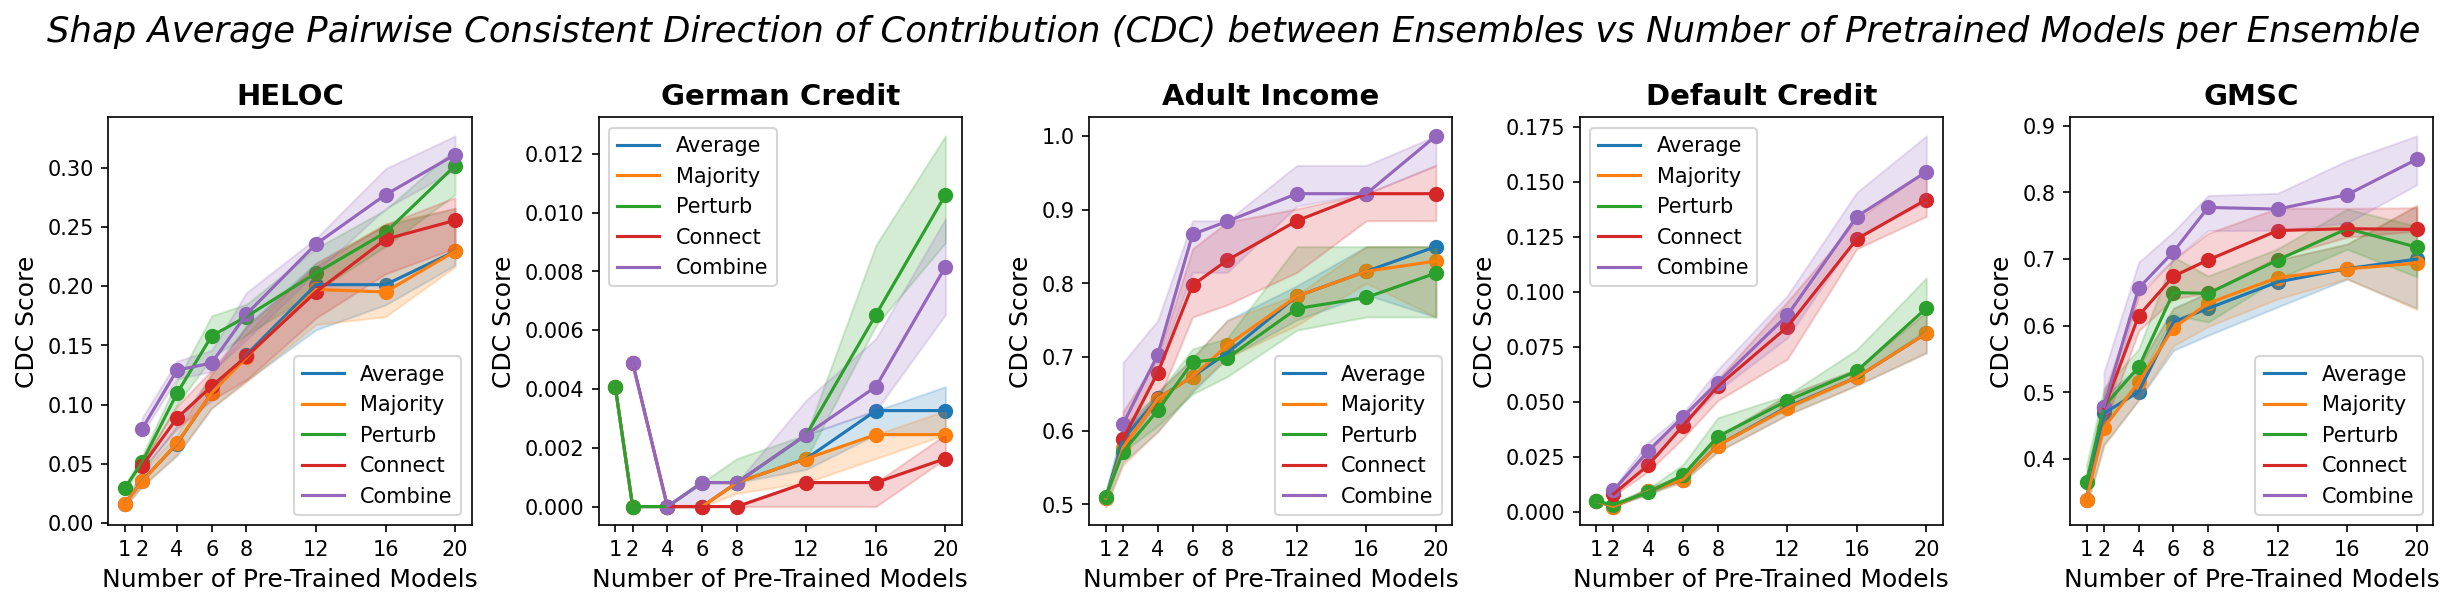
\includegraphics[width=0.99\textwidth]{figures/cdc_topd_shap.png}
    \caption{\small Effectiveness of ensemble strategies in stabilizing explanations across all datasets (top-5 SA, top-5 SSA, and top-$d$ CDC scores for \textbf{DeepSHAP}). \textit{Average} and \textit{Majority} denote vanilla ensembles, while \textit{Perturb}, \textit{Connect}, and \textit{Combine} denote weight perturbation, mode connectivity, and their combination respectively.}
    \label{fig:ensembles_all_shap}
\end{figure}

\section{Limitations and future work}
\label{app:limitations}

This work presents a novel approach to enhancing the consistency of model explanations by leveraging ensembling methods based on loss landscape exploration. While we observe promising results, we acknowledge that several interesting avenues for future work emerge from our study.

\paragraph{Underspecification set} In this work, we define the underspecification set as the collection of optimal models trained with a fixed set of hyperparameters, with the only source of variation due to the random seed using in training. By focusing on the underspecification set, we aim to shed light on the intrinsic inconsistency of model explanations arising purely from indeterminacy within a specific model configuration, rather than across different configurations.

However, we acknowledge that in real-world scenarios, an exact underspecification set may not always be found. Often, there are multiple sets of near-optimal hyperparameters, each potentially giving rise to a different underspecification set. The focus on one such set in our study is intentional, as it provides a clearer landscape for assessing the effectiveness of ensemble techniques in handling model indeterminacy. It is important to contextualize that addressing the complexities within the underspecification set is a necessary first step. Without a sound understanding of the explanatory behavior within a specific model configuration, attempting to reconcile explanations across broader ranges – such as the entire Rashomon set encompassing different model classes and hyperparameters – would be overly ambitious. Thus, our focus on the underspecification set offers an essential foundation for further research in the quest for more consistent model explanations.

Looking forward, an interesting direction for future work is the exploration of multiple underspecification sets concurrently. Comparing and consolidating explanations across multiple underspecification sets may present additional challenges but also provide further insights into the behavior of model explanations. This exploration would segue naturally into investigating the Rashomon set. Differing from the underspecification set, which captures the variation within a specific model configuration, a comprehensive exploration of the Rashomon set would entail an expanded understanding of the variance of model explanations.

\paragraph{Alternate explanation methods} We have chosen to use gradient-based methods for generating explanations in this study due to their simplicity, computational efficiency, and intuitive appeal. The gradient of a model with respect to its inputs can provide valuable insights about how the model responds to changes in those inputs. In essence, it can inform us about the local sensitivity of the model's predictions and thus can be interpreted as a form of local explanation method. Moreover, gradients can be seen as a natural proxy for counterfactual explanations (CEs), another popular category of explanation methods. CEs identify the minimal changes required in the input features to achieve a different prediction outcome. Because gradients indicate the direction of the greatest change in the model's output, they can be seen as giving a first approximation to CE directions.

However, it is worth noting that CEs, while providing a powerful intuitive appeal, come with their own set of challenges. They often require more computation than gradient-based methods, and they can be sensitive to the specific definition of ``minimal change'', which can depend on domain-specific factors. While we have focused on gradient-based explanations for their straightforwardness and direct relation to counterfactual reasoning, the field is open for further investigation and exploration of alternative methods for enhancing the consistency of model explanations.

We acknowledge that there is a wide array of explanation methods available, each with its unique advantages and limitations, and many of which could be considered in the context of our framework. Future work could explore other types of explanations, including counterfactual methods, or prototype-based methods, among others. Each of these could provide different perspectives on the consistency of model explanations and their susceptibility to model indeterminacy.

\paragraph{Weight perturbations and mode connectivity} We employ two strategies for navigating the loss landscape: local exploration via weight perturbations and global exploration via mode connectivity.

Weight perturbations could be perceived as the `safer' strategy, presenting a lower risk profile (dependent on the standard deviation of perturbations) but potentially hitting a performance ceiling based on dataset and model class (Section~\ref{subsec:experiments_weight} and Appendix~\ref{app:weights}). The performance of this method can be further optimized by considering a selection process for the perturbations, possibly based on training accuracy, or by adjusting the sampling strategy for the perturbation magnitude, taking into account the hyperspherical distribution of samples in high-dimensional weight space. On the other hand, mode connectivity may be perceived as `riskier' due to its broader scope but could yield benefits that go beyond the reach of simple local exploration, allowing us to explore more distant regions of the loss landscape, connecting different locally optimal solutions.

Looking ahead, there is much to learn and optimize about these methods. Future work would include both refining the methods of weight perturbation, and exploring alternate paths for mode connectivity \citep{ainsworth2023, gotmare2018, singh2020, tatro2020, zhao2020}, in order to develop better heuristics for navigating the loss landscape. The ultimate aim is to devise more effective strategies for ensemble creation that balance the goals of model performance, explanation consistency, and computational efficiency.

\paragraph{Improving inference efficiency} Although our methods require no extra training compared to standard ensembling, approaches to reduce the total number of models included in the set should be explored to cut inference costs.\footnote{Note additionally that our implementations may not be fully optimized with respect to parallelization, etc.} For instance, using ensembles with 10 pre-trained models each perturbed 50 times totals 500 models. While our methods offer computational efficiency compared to standard ensembling techniques with respect to the number of pre-trained models required, the practicality of this approach might still be challenging for larger scale applications. Future work could focus on finding efficient ways to reduce the total number of models in the ensemble. This could involve techniques such as weight permutations to align models and subsequently averaging the weights, or investigating methods to find a single weight configuration that matches the output of ensembles, which we detail in the following two paragraphs.

\paragraph{Exploring permutation symmetries} The initial investigations provided in this work could greatly benefit from the exploration of permutation symmetries. This emerging direction in research promises a more efficient traversal of the underspecification set \citep{ainsworth2023, singh2020, tatro2020}. The strategy involves aligning constituent models in weight space through permutation symmetries, thereby reducing the complexity of exploring numerous paths in the loss landscape. Through this approach, we hope to optimize the exploration process, enabling faster and more effective generation of ensembles. Not only would this strategy potentially reduce computational demands, it may also lead to uncovering more consistent explanations across ensembles, and aid in enhancing our understanding of model indeterminacy.

\paragraph{Consolidating ensemble models} The concept of consolidating ensembles into a single point in weight space stands as another promising direction for future work. The intention behind this proposed direction is to reap the benefits of ensemble modeling (explanation alignment, improved predictive performance, robustness against overfitting or dataset shift, etc.), while reducing the computational cost associated with operating large numbers of constituent models. Methods such as weight averaging~\citep{izmailov2018} or model fusion~\citep{singh2020} could potentially achieve this goal.

Furthermore, examining the effects of distillation and self-distillation could provide additional insights into model indeterminacy and the consistency of model explanations. Distillation techniques aim to compress the knowledge of an ensemble into a single, often simpler, model. Analyzing the impact of these techniques on the consistency and quality of explanations is an exciting prospect for future investigations. A connection to Bayesian methods might also be made, which inherently capture model uncertainty and can provide a measure of variability in single modes. However, these methods often face challenges related to computational efficiency and robustness to dataset shift. By contrast, ensemble methods can potentially offer a more widely accepted and practical alternative. The balance between ensemble techniques and Bayesian methods and their respective impacts on explanation consistency is worth considering.

\paragraph{Broader impact} The presented ensembling strategies for improving explanation consistency, while not explicitly designed to address issues of fairness or bias in AI models, have the potential for significant societal impact. It is expected that the insights gained from our methods will be beneficial for practitioners seeking to construct ML models that provide reliable explanations, which is especially crucial in fields where decision-making based on model outputs has high-stakes consequences, such as healthcare, finance, and criminal justice.

While the methods we showcase make strides in explanation consistency, they do not explicitly handle the problem of fairness and bias in AI, a concern that has been highlighted in numerous studies. Model explanations that are consistent across different models might still be biased or unfair if the underlying models or data exhibit these issues. Thus, it's important to supplement our techniques with methods explicitly designed to test for and mitigate bias and unfairness in AI models.

Moreover, our approach does not guarantee perfect explanation consistency, and there may be cases where explanations between models or different runs might still vary to a certain degree. This could have implications in scenarios where consistent explanations are particularly important, such as in the application of machine learning models in legal or healthcare contexts.

Given these broader impacts, it's crucial for practitioners applying our methods to be aware of these considerations. We recommend combining our ensembling techniques with existing and future fairness-aware methods and robust validation procedures to ensure comprehensive analysis of model explanations. As this field evolves, we encourage future research on how to effectively integrate consideration of explanation consistency, fairness, and bias in AI model development and evaluation.

\paragraph{Closing remarks} In conclusion, our work provides a foundation to pave the way for future research directions towards leveraging neural network research to improve our knowledge of explanations amidst model indeterminacy. Although ensemble methods feature prominently in the neural network analysis literature, their application with respect to model explanations has received very little attention. As stated, advances in loss landscape understanding and implications of model indeterminacy have emerged as recent, yet distinct developments, with the two fields existing almost in parallel. We emphasize once more that the aim of this work is to serve as a catalyst for their convergence, and bring about a unified exploration of both areas. Through initial alignment of these directions, we have shed light on the interplay between model indeterminacy and the consistency of model explanations.

Moving forward, a rich and promising set of research directions awaits. Further exploration of the loss landscape, particularly in the pursuit of expedited mode connectivity, or distillation techniques, stands as an intriguing prospect. These directions would build on recent advancements in the field and potentially lead to more effective and reliable model explanations. Additionally, the application of permutation symmetries to align model weights prior to averaging is another promising direction. Each of these techniques may not only improve computational efficiency but also enhance our understanding of the loss landscape and its relationship with model explanations. Such strategies are, in essence, leveraging the mathematical structure inherent in neural networks to expedite the exploration of the underspecification set and promote explanation consistency.

We believe that the pursuit of these directions will continue to push the frontiers of our understanding of explanation consistency in AI models, contributing positively to the development of reliable, trustworthy, and interpretable artificial intelligence systems.